%%% Verze pro jednostranný tisk:
\documentclass[11pt,a4paper]{report}
\usepackage[top=25mm,bottom=25mm,right=25mm,left=30mm,head=12.5mm,foot=12.5mm]{geometry}
\let\openright=\clearpage

%%% Pokud tiskneme oboustranně:
%\documentclass[11pt,a4paper,twoside,openright]{report}
%\usepackage[top=25mm,bottom=25mm,right=25mm,left=30mm,head=12.5mm,foot=12.5mm]{geometry}
%\let\openright=\cleardoublepage

%%% Definice různých užitečných maker (viz popis uvnitř souboru)
%%% Tento soubor obsahuje definice různých užitečných maker a prostředí %%%
%%% Další makra připisujte sem, ať nepřekáží v ostatních souborech.     %%%

\usepackage[a-2u]{pdfx}     % výsledné PDF bude ve standardu PDF/A-2u

\usepackage{ifpdf}
\usepackage{ifxetex}
\usepackage{ifluatex}

%%% Nastavení pro použití samostatné bibliografické databáze.
\usepackage[
   backend=biber
%  ,style=iso-authoryear
  ,style=numeric
  ,sortlocale=cs_CZ
  ,alldates=iso
  ,bibencoding=UTF8
  %,block=ragged
]{biblatex}
\let\cite\parencite
\bibliography{literatura}

%% Přepneme na českou sazbu, fonty Latin Modern a kódování češtiny
\ifthenelse{\boolean{xetex}\OR\boolean{luatex}}
   { % use fontspec and OpenType fonts with utf8 engines
			\usepackage[english,slovak,czech]{babel}
			\usepackage[autostyle,english=british,czech=quotes]{csquotes}
			\usepackage{fontspec}
			\defaultfontfeatures{Ligatures=TeX,Scale=MatchLowercase}
   }
   {
			\usepackage[english,slovak,czech]{babel}
			\usepackage{lmodern}
			\usepackage[T1]{fontenc}
			\usepackage{textcomp}
			\usepackage[utf8]{inputenc}
			\usepackage[autostyle,english=british,czech=quotes]{csquotes}
	 }
\ifluatex
\makeatletter
\let\pdfstrcmp\pdf@strcmp
\makeatother
\fi

%%% Další užitečné balíčky (jsou součástí běžných distribucí LaTeXu)
\usepackage{amsmath}        % rozšíření pro sazbu matematiky
\usepackage{amsfonts}       % matematické fonty
\usepackage{amssymb}        % symboly
\usepackage{amsthm}         % sazba vět, definic apod.
\usepackage{bm}             % tučné symboly (příkaz \bm)
\usepackage{graphicx}       % vkládání obrázků
\usepackage{listings}       % vylepšené prostředí pro strojové písmo
\usepackage{fancyhdr}       % prostředí pohodlnější nastavení hlavy a paty stránek
\usepackage{icomma}         % inteligetní čárka v matematickém módu
\usepackage{dcolumn}        % lepší zarovnání sloupců v tabulkách
\usepackage{booktabs}       % lepší vodorovné linky v tabulkách
\makeatletter
\@ifpackageloaded{xcolor}{
   \@ifpackagewith{xcolor}{usenames}{}{\PassOptionsToPackage{usenames}{xcolor}}
  }{\usepackage[usenames]{xcolor}} % barevná sazba
\makeatother
\usepackage{multicol}       % práce s více sloupci na stránce
\usepackage{caption}
\usepackage{enumitem}
\setlist[itemize]{noitemsep, topsep=0pt, partopsep=0pt}
\setlist[enumerate]{noitemsep, topsep=0pt, partopsep=0pt}
\setlist[description]{noitemsep, topsep=0pt, partopsep=0pt}

\usepackage{tocloft}
\setlength\cftparskip{0pt}
\setlength\cftbeforechapskip{1.5ex}
\setlength\cftfigindent{0pt}
\setlength\cfttabindent{0pt}
\setlength\cftbeforeloftitleskip{0pt}
\setlength\cftbeforelottitleskip{0pt}
\setlength\cftbeforetoctitleskip{0pt}
\renewcommand{\cftlottitlefont}{\Huge\bfseries\sffamily}
\renewcommand{\cftloftitlefont}{\Huge\bfseries\sffamily}
\renewcommand{\cfttoctitlefont}{\Huge\bfseries\sffamily}

% vyznaceni odstavcu
\parindent=0pt
\parskip=11pt

% zakaz vdov a sirotku - jednoradkovych pocatku ci koncu odstavcu na prechodu mezi strankami
\clubpenalty=1000
\widowpenalty=1000
\displaywidowpenalty=1000

% nastaveni radkovani
\renewcommand{\baselinestretch}{1.20}

% nastaveni pro nadpisy - tucne a bezpatkove
\usepackage{sectsty}    
\allsectionsfont{\sffamily}

% nastavení hlavy a paty stránek
\fancyhf{}
%\fancyhead[RO,LE]{\rightmark}
\fancyfoot[RO]{\thepage}
\renewcommand{\footrulewidth}{.5pt}
\fancypagestyle{plain}{%
\fancyhf{} % clear all header and footer fields
\fancyfoot[RO,LE]{\thepage}
\renewcommand{\headrulewidth}{0pt}
\renewcommand{\footrulewidth}{0.5pt}}

% Tato makra přesvědčují mírně ošklivým trikem LaTeX, aby hlavičky kapitol
% sázel příčetněji a nevynechával nad nimi spoustu místa. Směle ignorujte.
\makeatletter
\def\@makechapterhead#1{
  {\parindent \z@ \raggedright \sffamily
   \Huge\bfseries \thechapter. #1
   \par\nobreak
   \vskip 20\p@
}}
\def\@makeschapterhead#1{
  {\parindent \z@ \raggedright \sffamily
   \Huge\bfseries #1
   \par\nobreak
   \vskip 20\p@
}}
\makeatother

% Trochu volnější nastavení dělení slov, než je default.
\lefthyphenmin=2
\righthyphenmin=2

% Zapne černé "slimáky" na koncích řádků, které přetekly, abychom si
% jich lépe všimli.
\overfullrule=1mm

%% Balíček hyperref, kterým jdou vyrábět klikací odkazy v PDF,
%% ale hlavně ho používáme k uložení metadat do PDF (včetně obsahu).
%% Většinu nastavítek přednastaví balíček pdfx.
\hypersetup{unicode}
\hypersetup{breaklinks=true}
\hypersetup{hidelinks}

%%% Prostředí pro sazbu kódu, případně vstupu/výstupu počítačových
%%% programů. (Vyžaduje balíček listings -- fancy verbatim.)
\lstnewenvironment{code}{\lstset{basicstyle=\small, frame=single}}{}

\usepackage{algpseudocode}
\usepackage{algorithm}

\usepackage{listings, xcolor}
\lstset{
tabsize = 4,
showstringspaces = false,
commentstyle = \color{black},
keywordstyle = \color{blue},
stringstyle = \color{red},
basicstyle = \scriptsize \ttfamily,
breaklines = true,
numberstyle = \tiny,
}

\lstdefinelanguage{turtle}
{
columns=fullflexible,
keywordstyle=\color{red},
morekeywords={@prefix,@base,@forSome,@forAll,@keywords},
morecomment=[l]{\#},
tabsize=4,
alsoletter={-?}, % allowed in names
morecomment=[s][\color{blue}]{<}{>},
%basicstyle=\ttfamily\color{black},
%numberstyle=\color{black},
morestring=[b][\color{black}]\",
}
\usepackage{numprint}

\usepackage{multirow}
\usepackage{colortbl}
\usepackage{hhline}
%\usepackage[table,xcdraw]{xcolor}

%%% DEFINICE ZÁKLADNÍCH PROMĚNNÝCH
\def\TypPrace{BP}                % bakalářská práce/bachelor thesis
%\def\TypPrace{DP}               % diplomová práce/master thesis
%\def\Jazyk{cze}                  % čeština/czech
%\def\Jazyk{slo}                 % slovenština/slovak
\def\Jazyk{eng}                 % angličtina/english

%%% Název práce v jazyce práce (přesně podle zadání)
%%% Title of the thesis in the language used in the text (exact according to assignment)
\def\NazevPrace{Název práce}

%%% Tento soubor obsahuje definice různých užitečných maker a prostředí %%%
%%% Další makra připisujte sem, ať nepřekáží v ostatních souborech.     %%%

\usepackage[a-2u]{pdfx}     % výsledné PDF bude ve standardu PDF/A-2u

\usepackage{ifpdf}
\usepackage{ifxetex}
\usepackage{ifluatex}

%%% Nastavení pro použití samostatné bibliografické databáze.
\usepackage[
   backend=biber
%  ,style=iso-authoryear
  ,style=numeric
  ,sortlocale=cs_CZ
  ,alldates=iso
  ,bibencoding=UTF8
  %,block=ragged
]{biblatex}
\let\cite\parencite
\bibliography{literatura}

%% Přepneme na českou sazbu, fonty Latin Modern a kódování češtiny
\ifthenelse{\boolean{xetex}\OR\boolean{luatex}}
   { % use fontspec and OpenType fonts with utf8 engines
			\usepackage[english,slovak,czech]{babel}
			\usepackage[autostyle,english=british,czech=quotes]{csquotes}
			\usepackage{fontspec}
			\defaultfontfeatures{Ligatures=TeX,Scale=MatchLowercase}
   }
   {
			\usepackage[english,slovak,czech]{babel}
			\usepackage{lmodern}
			\usepackage[T1]{fontenc}
			\usepackage{textcomp}
			\usepackage[utf8]{inputenc}
			\usepackage[autostyle,english=british,czech=quotes]{csquotes}
	 }
\ifluatex
\makeatletter
\let\pdfstrcmp\pdf@strcmp
\makeatother
\fi

%%% Další užitečné balíčky (jsou součástí běžných distribucí LaTeXu)
\usepackage{amsmath}        % rozšíření pro sazbu matematiky
\usepackage{amsfonts}       % matematické fonty
\usepackage{amssymb}        % symboly
\usepackage{amsthm}         % sazba vět, definic apod.
\usepackage{bm}             % tučné symboly (příkaz \bm)
\usepackage{graphicx}       % vkládání obrázků
\usepackage{listings}       % vylepšené prostředí pro strojové písmo
\usepackage{fancyhdr}       % prostředí pohodlnější nastavení hlavy a paty stránek
\usepackage{icomma}         % inteligetní čárka v matematickém módu
\usepackage{dcolumn}        % lepší zarovnání sloupců v tabulkách
\usepackage{booktabs}       % lepší vodorovné linky v tabulkách
\makeatletter
\@ifpackageloaded{xcolor}{
   \@ifpackagewith{xcolor}{usenames}{}{\PassOptionsToPackage{usenames}{xcolor}}
  }{\usepackage[usenames]{xcolor}} % barevná sazba
\makeatother
\usepackage{multicol}       % práce s více sloupci na stránce
\usepackage{caption}
\usepackage{enumitem}
\setlist[itemize]{noitemsep, topsep=0pt, partopsep=0pt}
\setlist[enumerate]{noitemsep, topsep=0pt, partopsep=0pt}
\setlist[description]{noitemsep, topsep=0pt, partopsep=0pt}

\usepackage{tocloft}
\setlength\cftparskip{0pt}
\setlength\cftbeforechapskip{1.5ex}
\setlength\cftfigindent{0pt}
\setlength\cfttabindent{0pt}
\setlength\cftbeforeloftitleskip{0pt}
\setlength\cftbeforelottitleskip{0pt}
\setlength\cftbeforetoctitleskip{0pt}
\renewcommand{\cftlottitlefont}{\Huge\bfseries\sffamily}
\renewcommand{\cftloftitlefont}{\Huge\bfseries\sffamily}
\renewcommand{\cfttoctitlefont}{\Huge\bfseries\sffamily}

% vyznaceni odstavcu
\parindent=0pt
\parskip=11pt

% zakaz vdov a sirotku - jednoradkovych pocatku ci koncu odstavcu na prechodu mezi strankami
\clubpenalty=1000
\widowpenalty=1000
\displaywidowpenalty=1000

% nastaveni radkovani
\renewcommand{\baselinestretch}{1.20}

% nastaveni pro nadpisy - tucne a bezpatkove
\usepackage{sectsty}    
\allsectionsfont{\sffamily}

% nastavení hlavy a paty stránek
\fancyhf{}
%\fancyhead[RO,LE]{\rightmark}
\fancyfoot[RO]{\thepage}
\renewcommand{\footrulewidth}{.5pt}
\fancypagestyle{plain}{%
\fancyhf{} % clear all header and footer fields
\fancyfoot[RO,LE]{\thepage}
\renewcommand{\headrulewidth}{0pt}
\renewcommand{\footrulewidth}{0.5pt}}

% Tato makra přesvědčují mírně ošklivým trikem LaTeX, aby hlavičky kapitol
% sázel příčetněji a nevynechával nad nimi spoustu místa. Směle ignorujte.
\makeatletter
\def\@makechapterhead#1{
  {\parindent \z@ \raggedright \sffamily
   \Huge\bfseries \thechapter. #1
   \par\nobreak
   \vskip 20\p@
}}
\def\@makeschapterhead#1{
  {\parindent \z@ \raggedright \sffamily
   \Huge\bfseries #1
   \par\nobreak
   \vskip 20\p@
}}
\makeatother

% Trochu volnější nastavení dělení slov, než je default.
\lefthyphenmin=2
\righthyphenmin=2

% Zapne černé "slimáky" na koncích řádků, které přetekly, abychom si
% jich lépe všimli.
\overfullrule=1mm

%% Balíček hyperref, kterým jdou vyrábět klikací odkazy v PDF,
%% ale hlavně ho používáme k uložení metadat do PDF (včetně obsahu).
%% Většinu nastavítek přednastaví balíček pdfx.
\hypersetup{unicode}
\hypersetup{breaklinks=true}
\hypersetup{hidelinks}

%%% Prostředí pro sazbu kódu, případně vstupu/výstupu počítačových
%%% programů. (Vyžaduje balíček listings -- fancy verbatim.)
\lstnewenvironment{code}{\lstset{basicstyle=\small, frame=single}}{}

\usepackage{algpseudocode}
\usepackage{algorithm}

\usepackage{listings, xcolor}
\lstset{
tabsize = 4,
showstringspaces = false,
commentstyle = \color{black},
keywordstyle = \color{blue},
stringstyle = \color{red},
basicstyle = \scriptsize \ttfamily,
breaklines = true,
numberstyle = \tiny,
}

\lstdefinelanguage{turtle}
{
columns=fullflexible,
keywordstyle=\color{red},
morekeywords={@prefix,@base,@forSome,@forAll,@keywords},
morecomment=[l]{\#},
tabsize=4,
alsoletter={-?}, % allowed in names
morecomment=[s][\color{blue}]{<}{>},
%basicstyle=\ttfamily\color{black},
%numberstyle=\color{black},
morestring=[b][\color{black}]\",
}
\usepackage{numprint}

\usepackage{multirow}
\usepackage{colortbl}
\usepackage{hhline}
%\usepackage[table,xcdraw]{xcolor}

%%% Jméno autora
%%% Author's name - First name Surname
\def\AutorPrace{Jméno Příjmení}

%%% Rok odevzdání a měsíc (slovně)
%%% Year of surrender and month (verbally) - month YYYY
\def\DatumOdevzdani{měsíc RRRR}

%%% Vedoucí práce: Jméno a příjmení s~tituly
%%% Supervisor: First name and surname with titles
\def\Vedouci{Vedoucí práce}

%%% Studijní program
%%% Study program
\def\StudijniProgram{studijní program}

%%% Studijní obor
%%% Field of study
\def\StudijniObor{studijní obor}

%%% Nepovinné poděkování (vedoucímu práce, konzultantovi, tomu, kdo zapůjčil software, literaturu apod.)
%%% Optional thanks (the supervisor, the consultant, the borrower of software, literature, etc.)
\def\Podekovani{%
Poděkování.
}

%%% Abstrakt (doporučený rozsah cca 150-250 slov; nejedná se o zadání práce)
\def\Abstrakt{%
Abstrakt.
}
\def\AbstraktEN{%
Abstract.
}

%%% 3 až 5 klíčových slov (doporučeno)
\def\KlicovaSlova{klíčové slovo, další pojem, jiný důležitý termín, a ještě jeden}
\def\KlicovaSlovaEN{keyword, important term, another topic, and another one}

%%% Titulní strana a různé povinné informativní strany
%%% Title page and various mandatory information pages
\begin{document}
%%%% Titulní strana práce a další povinné informační strany

%%% Titulní strana práce

\pagestyle{empty}
\hypersetup{pageanchor=false}

\begin{center}
\Huge\sffamily
\VSE\\
\FIS

\vspace{\stretch{1}}


\includegraphics[width=.3\textwidth]{img/logo-FIS}

\vspace{\stretch{2}}

\bfseries\NazevPrace

\vspace{8mm}
\mdseries\TypPraceText

\vspace{8mm}
\large
\begin{tabular}{rl}
\StudijniProgramText: & \StudijniProgram \\
\noalign{\vspace{2mm}}
\StudijniOborText: & \StudijniObor \\
\end{tabular}

\vspace{\stretch{8}}

\begin{tabular}{rl}
\AutorText: & \AutorPrace \\
\noalign{\vspace{2mm}}
\VedouciText: & \Vedouci \\
\end{tabular}

\vspace{8mm}
\Praha, \DatumOdevzdani
\end{center}


%%% Poděkování
\hypersetup{pageanchor=true}
\cleardoublepage
\pagestyle{plain}
\openright
\vspace*{\fill}
\section*{\PodekovaniText}
\noindent
\Podekovani
\vspace{1cm}


%%% Povinná informační strana bakalářské práce
\openright
\section*{Abstrakt}
\noindent
\Abstrakt
\subsection*{Klíčová slova}
\noindent
\KlicovaSlova

\bigskip\bigskip\bigskip
\section*{Abstract}
\noindent
\AbstraktEN
\subsection*{Keywords}
\noindent
\KlicovaSlovaEN

\openright


%%% Strana s automaticky generovaným obsahem práce
%%% A page with automatically generated content of the thesis
\setcounter{tocdepth}{2}
\tableofcontents

%%% Seznam obrázků v práci
%%% List of figures in the thesis
\openright
%\listoffigures

%%% Seznam tabulek v práci (volitelně)
%%% List of tables in the thesis (optionally)
\clearpage
%\listoftables

%%% Seznam zkratek v práci (volitelně)
%%% List of abbreviations in the thesis (optionally)
%\chapter*{\SeznamZkratek}

\begin{multicols}{2}
\raggedright
\begin{description}
\item [BCC] Blind Carbon Copy
\item [CC] Carbon Copy
\item [CERT] Computer Emergency Response Team
\item [CSS] Cascading Styleheets
\item [DOI] Digital Object Identifier
\item [HTML] Hypertext Markup Language
\item [REST] Representational State Transfer
\item [SOAP] Simple Object Access Protocol
\item [URI] Uniform Resource Identifier
\item [URL] Uniform Resource Locator
\item [XML] eXtended Markup Language
\end{description}
\end{multicols}



\pagestyle{fancy}
%%% Jednotlivé kapitoly práce jsou pro přehlednost uloženy v samostatných souborech
%%% The individual chapters of the thesis are stored in separate files for clarity
%\chapter*{Introduction}
\addcontentsline{toc}{chapter}{Introduction}

OLAP \cite{berson1997} or data cubes are established as one of the standard tools for analysing aggregated data and are an essential part of any Bussiness Intelligence solution. Any transactional data, that relates to multiple contexts (e.g. multinational fast food chain's sales can be divided with respect to regions, marketing campaigns etc.) can be transformed into their multidimensional representation in a form of OLAP cube where the contexts potentially relevant for analysis make up the dimensions of the cube and be examined in one of many available standard BI tools (such as Microsoft Excel, Power BI etc.), that facilitate aggregation of the values and manipulation with the cube in order to gain insights into the data.

Data mining can function as an alternative or complement \cite{Chudan2015} to OLAP analysis. The term data mining refers to extracting or \textit{mining} knowledge from large amounts of data (Hand et al.,2001 TODO cite), usually relational databases where the data is on the most granular level. The purpose of data mining is either \textit{descriptive}, where it is aimed to find and describe regularities and patterns in the data, or \textit{predictive}, where the goal is to infere new information hidden in the data, that can be used to make predictions. Association rules are on of the data mining methods and can be used for descriptive and predictive analysis. The rules can be mined by different algorithms, namely Apriori algorithm \cite{Agrawal1993} and the ASSOC procedure of the GUHA method.\cite{hajek1966} They both serve to mine association rules in tabular data.

Data representation is not only limited to tables. In the environment of World Wide Web, data that is intented to be published to the public, is often modelled according to the Resource Description Framework (RDF) model. Individual records in the RDF model take a form of \textit{triples}, that represent binary relationships between the described entities. Sets of the relationships between entities and concepts that those entities can represent are call \textit{vocabularies} or \textit{ontologies} and are published as RDF as well. The relationships can connect entities from different data sources, making the data \textit{linked}. The term \textit{Linked Open data} (LOD) has become established for RDF data, which adheres to the use of standard formats, technologies and interconnection principles that facilitate and expand the possibilities of working with this data. 

An algorithm, that was designed specifically for the purposes of mining rules similar to association rules from the RDF data in the Web environment, is called \textit{\textbf{A}ssociation Rule \textbf{M}ining under \textbf{I}ncomplete \textbf{E}vidence}, shorty AMIE. \cite{Galarraga2013} Since the release of the original version of the algorithm, its original authors have published its two extensions, called AMIE+ \cite{Galarraga2015} and AMIE 3 \cite{Galarraga2020}, respectively. Another extension that builds on the AMIE + version, called RDFRules \cite{Zeman2020}, comes with its reference implementation in the form of a robust framework, which focuses not only on the rule mining itself but also on the possible preprocessing of input data and processing the generated rules.

Public-sector organizations and governmental bodies, that manage a large amount of data including various registers and demographic and economic statistics are often incentivised to publish some of their data for the benefit of their citizens. Due to the data privacy restrictions \cite{gdpr162_2020}, the organisations often resort to publish their data in an aggregated form. Some of the organizations, such as the European Union through its \textit{OpenBudgets.eu}\footnote{\href{https://ec.europa.eu/digital-single-market/en/content/openbudgetseu}{https://ec.europa.eu/digital-single-market/en/content/openbudgetseu}} platform or the Czech Social Security Administration\footnote{\href{https://data.cssz.cz/}{https://data.cssz.cz/}}, acknowledge the advantages of publishing their data in a universal and standard way for the consumers and do not hesitate to devote their resources to publishing their data as LOD. The Data Cube vocabulary \cite{dcv2014} is used to write aggregated data in the form of a data cube in the RDF model.

The interlinked nature of LOD encourages the published data cubes to be enriched with additional information available from other sources published as RDF as well. The connection would be made through those data cube dimension values that simultaneously occur as objects in large cross-domain LOD data set known as \textit{knowledge graphs}. Those can be municipalities, regions, organizations, products, etc. This new information in the form of binary relationships contained in these knowledge graphs can be used to mine association rules over the aggregated data, which can lead to finding relationships that cannot be found in the cubes themselves. Mining of association rules over RDF data and at the same time in their aggregated form is a not yet explored area and achieving generation of meaningful interpretable rules that bring new knowledge is a not yet solved problem.

The goals of this work are to:

\begin{enumerate}
    \item explore the possibilities of enriching RDF data cube structured by the Data Cube vocabulary with the data from general knowledge graphs and of mining such data by the AMIE algorithm or its derivatives,
    \item carry out an experiment that would demonstrate that such approach is possible and capable of yielding new interesting insights on the aggregated data. 
\end{enumerate}

The RDFRules framework is one of the tools used for performing the experiment. The aggregated data examined in the experiment are Czech pension statistics published by Czech Social Security Administration and Czech demography statistics of the Czech statistical office\footnote{\href{https://www.czso.cz/csu/czso/home}{https://www.czso.cz/csu/czso/home}}. The triples associated with the dimension values of the data cube are extracted from Wikidata\footnote{\href{https://www.wikidata.org/}{https://www.wikidata.org/}} and YAGO\footnote{\href{https://yago-knowledge.org/}{https://yago-knowledge.org/}} knowledge graphs.

This paper is organised as follows. Section \ref{linkeddata} provides an overview of Linked Open Data principles, RDF data model and its serialization formats, and the data sets used in the experiment. Section \ref{datacubes} introduces the basic concepts of OLAP cubes and describes the vocabularies used for representing the data cubes in RDF. Section \ref{assocrules} explains the basics of the association rule mining. Section \ref{amieandits} describes the AMIE algorithm, the improvements of its extension AMIE+ and presents the improvements of RDFRules algorithm and the techniques suggested to be used along with it. Section \ref{rdfrules} describes the reference implementation of the RDFRules. Section \ref{combining} elaborates the possibilities and implications of mining rules over RDF data cubes with combination of triples from knowledge graphs. Section \ref{experiment} describes thoroughly the performed experiment. Section \ref{discussion} elaborates the results of the executed mining tasks and encountered problems and the conclusion summarizes the contribution of the work and gives suggestions for further activities.

% i vysvětlení, co bude v dalších kapitolách jako „preliminaries“ – linked data, data cubes a dolování pravidel

% co je v kapitole 4 (ze tam jsou algoritmy které vysvetlují background frameworku RDFRules), kapitola 5 je o frameworku, kapitola 6, kapitola 7, kapitola 8
\chapter{Linked Data}

Linked Data is a set of best practices for publishing and connecting data on the Web structured in such a way that it is usable not only for human processing but also processable by machines. It builds upon the general architecture of the World Wide Web. Instead of creating links between particular documents from different sources in the case of the classic Web of documents, the Linked Data connects the representations of real-world objects or abstract concepts. Tim Berners-Lee expressed these best practises in four principles, known as the Linked Data principles.\cite{bernersLee2006}

\begin{itemize}
    \item Use URIs as names for things.
    \item Use HTTP URIs, so that people can look up those names.
    \item When someone looks up a URI, provide useful information, using the standards
    \item Include links to other URIs, so that they can discover more things.
\end{itemize}

URIs (Universal Resource Identifier) are used to identify real-world objects and abstract concepts. According to the second principle, information about the entity that the URI represents can be retrieved using HTTP protocol (so-called URI dereferencing). Based on the third principle, which advocates for a standard structure of data dereferenceable by URI, the Resource Description Framework (RDF) has been designed. Tim Berners-Lee also suggested 5-star deployment scheme for ranking published data according to the format in which it is published, comparing them based on their ability to be machine processed. It assigns one star to any data published and assigns the highest number of five stars to data, that is published as RDF, where the entities described are identified by an dereferenceable URI string and the data are connected to other data sources.

\section{Resource Description Framework}

RDF is a data model based on representing data as directed graphs. The basic building block of RDF structured data is a triple consisting of three parts called subject, predicate, and object. The subject is the URI representing the described resource. The object is either URI or literal value like string or number. The predicate specifies the type of relationship between the resources at the positions of subject and object. The predicate is always identified by URI. Predicate URIs come from vocabularies, intended to encompass various relations and concepts occurring in a certain domain.

Set of triples then establishes a RDF graph. URIs at the subject and object positions of the triples make nodes of the graph and each triple acts as an arc connecting the nodes. Type of the connecting is expressed by the predicate URI in the triple. Given the uniqueness of the URIs and their capability of being dereferenced and connected to URIs from various sources (the fourth Linked Data principle), one can imagine the linked data as one giant undivided graph containing data from various topical domains, so-called Web of Data.

It is important to distinguish the model itself from its formats. RDF describes only an abstract structure of the data that has to be materialized into a certain format when the data is published on the Web. The first standard serialization format published together with RDF in \cite{rdfPrimer2004} is RDF/XML. An example of two triples described in RDF/XML format is shown in the listing \ref{rdfxmlexample}. The RDF/XML format suits well the use cases, where little human interaction with the data is expected because its syntax is difficult for a human to read and write compared to other formats. On the other hand, its XML background makes it a perfect format for data processed and generated solely by machines.

\begin{figure}[h]
\begin{lstlisting}[language = XML, caption={Example of RDF data described in RDF/XML format (Source: author)}, label={rdfxmlexample},captionpos=b escapeinside={(*@}{@*)}]
<?xml version="1.0" encoding="UTF-8"?>
<rdf:RDF
    xmlns:rdf="http://www.w3.org/1999/02/22-rdf-syntax-ns#"
    xmlns:foaf="http://xmlns.com/foaf/0.1/">
    <rdf:Description rdf:about="http://example.com/john-johnson">
        <rdf:type rdf:resource="http://xmlns.com/foaf/0.1/Person"/>
        <foaf:name>John Johnson</foaf:name>
    </rdf:Description>
</rdf:RDF>
\end{lstlisting}
\end{figure}

One of the most used and most human-readable formats is Turtle (Tense RDF Triple Language).\cite{turtlew3c2014} It provides various shorthands, enabling to make the representation as brief as possible and thus suitable to be written by hand. The common part of URI strings can be prefixed, so only the decisive end of the URIs has to be stated. The symbol of the semicolon is used to divide pairs of predicate and object belonging to the same subject, so the subject does not have to be repeated. If the described triples share both subject and predicate, a comma can be used to divide the different objects of the triples. Usage of a prefix and the two symbols is shown in an example in the listing \ref{turtleexample}.

\begin{figure}[h]
\begin{lstlisting}[language = turtle, caption={Example of RDF data described in Turtle format (Source: author)}, label={turtleexample},captionpos=b escapeinside={(*@}{@*)}]
@prefix rdf: <http://www.w3.org/1999/02/22-rdf-syntax-ns#> .
@prefix foaf: <http://xmlns.com/foaf/0.1/> .
@prefix eg: <http://example.com/> .
eg:john-johnson rdf:type foaf:Person ;
                             foaf:name "John Johnson" ;
                             foaf:knows eg:john-jackson, eg:jack-johnson .
\end{lstlisting}
\end{figure}

Same as with the relational data model and SQL, RDF also needs a capable language for querying and manipulating the data. For this purposes, SPARQL was designed.\cite{sparqlw3c2008} Example of a simple SELECT query written is SPARQL is shown in the listing \ref{sparqlexample}. Similarly to SQL, the WHERE clause serves to limit the search place from which the result of the query is given. Content of the WHERE clause resembles the Turtle syntax. URIs, that can be bound to variable that occurs in the pattern stated in the WHERE clause, are contained in the output of the query if the variable is enumerated after the SELECT keyword. This particular query would return all possible bindings for variable \verb|name| ie. all names of persons, for whom the queried data states, that they know a certain John Jackson.

\begin{figure}[h]
\begin{lstlisting}[language = SPARQL, caption={Example of a simple SPARQL query (Source: author)}, label={sparqlexample},captionpos=b escapeinside={(*@}{@*)}]
PREFIX rdf: <http://www.w3.org/1999/02/22-rdf-syntax-ns#>
PREFIX foaf: <http://xmlns.com/foaf/0.1/>
PREFIX eg: <http://example.com/>

select ?name where {
    ?person rdf:type foaf:Person ;
            foaf:name ?name ;
            foaf:knows eg:john-jackson .
}
\end{lstlisting}
\end{figure}

% TODO SPARQL endpoints

\section{Linked Open Data}

The first activities with the goal of starting the publication of Linked Data on a global scale were conducted by the Semantic Web research community as part of the W3C Linking Open Data (LOD) project established in 2007.\cite{Heath2011} The aim of the project was to identify datasets published under an open license and to publish them according to the Linked Data principles. All data sets that are published under an open license and are connected to other data sets are referred to as LOD cloud. 

The content of the LOD spans across multiple domains. The website \href{http://lod-cloud.net}{lod-cloud.net} tracks the current state of published LOD data sets and divides the data sets into these categories, so-called subclouds: Cross-Domain, Geography, Government, Life Sciences, Linquistics, Media, Publications, Social Networking and User-Generated. A data set can fall into more than one category. Cross-Domain, general knowledge data sets play an important role of an intermediary through which unrelated data sets can be connected. 

One of those data sets is Wikidata. It is a sister project of Wikipedia, founded and hosted by the Wikimedia Foundation. The data set is managed in an open an collaborative way. Everybody who is interested in expanding the knowledge base can create an account and start contributing. The website of the project provides an intuitive user interface for editing and creating data, so no technical skills beyond common usage of the Internet is needed. The data set currently contains over 93 million items edited by over 26 thousand active contributors. Every item of the dataset is allocated an unique identifier prefixed by the letter \textbf{Q}, so-called QID or Q number. The items are described by their statements corresponding to RDF triples. Predicates are in the context of Wikidata called properties and are prefixed by letter \textbf{P} similar to items. A sample of the triples contained in Wikidata in Turtle syntax shows listing \ref{wikidataexample}.

\begin{figure}[h]
\begin{lstlisting}[language = Turtle, caption={Wikidata content sample (Source: author)}, label={wikidataexample},captionpos=b escapeinside={(*@}{@*)}]
@prefix rdf: <http://www.w3.org/1999/02/22-rdf-syntax-ns#> .
@prefix wd: <http://www.wikidata.org/entity/> .
@prefix wdt: <http://www.wikidata.org/prop/direct> .
@prefix schema: <http:schema.org/> .

wd:Q111 wdt:P361 wd:Q7879772
        rdf:label "Mars" ;
        schema:description "fourth planet from the Sun";
\end{lstlisting}
\end{figure}

An different approach is taken by the DBpedia project. Instead of relying on manual contribution of volunteers, DBpedias data comes from an application of NLP extraction algorithms over plain text of Wikipedia's articles. 

% The facts of an RDF KB can usually be divided into an A-Box and a T-Box. While the A-Box contains instance data, the T-Box is the subset of facts that define classes, domains, ranges for predicates, and the class hierarchy.


%\begin{enumerate}
%    \item A unifying data model
%    \item A standardized data access mechanism
%    \item Hyperlink-based data discovery
%    \item Self-descriptive data -> If an application consuming Linked Data encounters data described with an unfamiliar vocabulary, the application can dereference the URIs that identify vocabulary terms in order to find their definition.
%\end{enumerate}


%The prototypical example of cross-domain Linked Data is DBpedia 6 -> wikidata, YAGO = cross-domain datasets

%Because of its breadth of topical coverage, DBpedia has served as a hub within the Web of Data from the early stages of the Linking Open Data project.

%Further cross-domain data sets include UMBEL 8 , YAGO [104], and OpenCyc 9 . These are, in turn, linked with DBpedia, helping to facilitate data integration across a wide range of interlinked sources.

%Geography is another factor that can often connect information from varied topical domains. This is apparent in the Web of Data, where the Geonames 10 data set frequently serves as a hub for other data sets that have some geographical component. Geonames is an open-license geographical database that publishes Linked Data about 8 million locations.

%Governmental bodies and public-sector organisations produce a wealth of data, ranging from economic statistics, to registers of companies and land ownership, reports on the performance of schools, crime statistics, and the voting records of elected representatives. Recent drives to \textbf{increase government transparency} have led to a significant increase in the amount of governmental and public-sector data that is made accessible on the Web.

%The potential of Linked Data for easing the access to government data is increasingly understood, with both the data.gov.uk 26 and data.gov 27 initiatives publishing significant volumes of data in RDF.
\chapter{Data Cubes\label{datacubes}}

While relational databases with highly normalized data models fit well to situations where data is frequently modified, they can be quite cumbersome when being performed complex aggregating queries. Online Analytical Processing (OLAP) system fits better these purposes. 

\section{Terminology}

In an OLAP system, numerical data is stored in a multidimensional data structure. The structure is comprised of hypothetical cells, called \textit{observations}, which are identified by their assigned set of \textit{dimension} values from each dimension of the structure. Each observation can contain zero to many numerical values, so-called \textit{measurements}. The meaning of the measurements is referred to as \textit{measure}. In the OLAP context the units of measure are called \textit{attributes}. The structure is referred to as OLAP Cube or Data Cube. The word \textit{cube} implies exactly three dimensions, but its purpose is only to illustrate the multidimensionality of the structure.

Distinct values of a dimension can be organized into a hierarchy, where the parent value is assigned to summarized measurements throughout its child values for each measure. An example of such a hierarchy could be a relationship of a product category and specific products belonging to this category. The depth of a dimension value in its hierarchy then determines the level of granularity the measurement values in a cell assigned to the dimension value are associated with. A cell with all dimension values at the lowest level in their hierarchies or in no hierarchy at all has the finest level of granularity. In a Data Cube consisting of only one cell, meaning each dimension of the cube has only one distinct value, the cell has the coarsest level of granularity.

\section{Operations}

Several operations can be performed on a Data Cube:

\begin{description}
    \item[roll-up] This operation aggregates data either by reduction of one or more dimensions or by climbing up a concept hierarchy for a dimension.
    \item[drill-down] This operation transforms data to a more detailed level. It is the opposite of roll-up operation. Either a new dimension is added or the values are projected on a more granular level of a dimension.
    \item[slice and dice] By slicing a cube only certain subset of the dimension values of one dimension is allowed in the resulting cube. Dicing means restricting dimension values across multiple dimensions.
    \item[pivot] Pivoting means rotating the cube by its axis in order to change the view of the data.
\end{description}

If the values contained in the cube have an additive character (e.g. sales amount or a number of security incidents), the values can be rolled up or drilled down along any dimension. Not all facts are additive though (e.g. average temperature). The analytical process itself lies in performing the above-mentioned operations in order to find interesting insight into the data. By precomputing the aggregations of all possible subsets of dimensions from the cube on the finest level of granularity, the whole process can be accelerated.

\section{The Data Cube Vocabulary\label{dcv}}

The principle of dimensions, measures and attributes are the basic building blocks of the standards and guidelines presented by the SDMX (Statistical Data and Metadata eXchange) initiative, that tries to standardize and modernize the exchange of statistical data. The World Wide Web Consortium's recommendation for representing multi-dimensional data in RDF is the Data Cube vocabulary.\cite{dcv2014} This vocabulary underlies the standards and guidelines of the SDMX initiative. It allows to publish the content of the cube together with information about its structure and its metadata. The structure of the vocabulary is shown in the picture \ref{qbstructureimg}.

\begin{figure}[h]
\centering
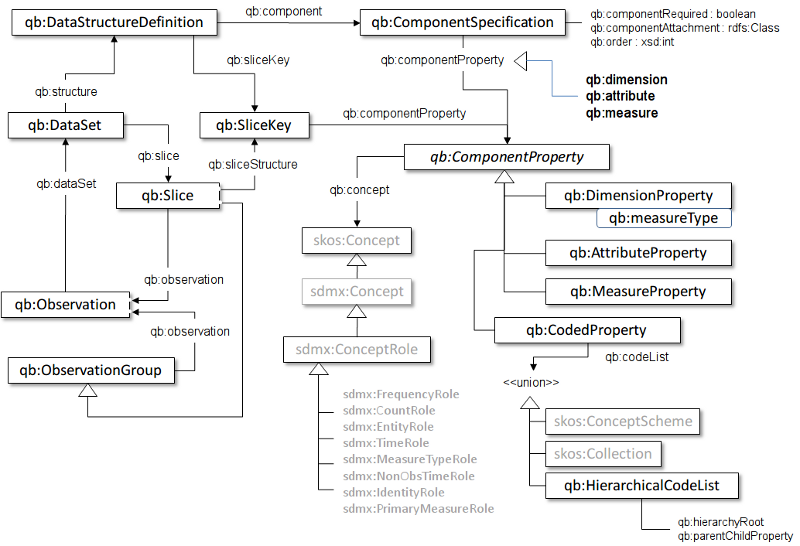
\includegraphics[width=0.8\textwidth]{img/qbstructure.png}
\caption{The Data Cube Vocabulary structure (Source: \cite{dcv2014})}
\label{qbstructureimg}
\end{figure}

The listing \ref{dcvobs1} shows an example of an observation represented with the Data Cube Vocabulary. The observation has a property $qb:dataSet$ which links it to the entity of the whole cube. The observation is assigned two measures $measure1$ and $measure2$ and is associated with dimension values of two cube's dimensions.

\begin{figure}[h]
\begin{lstlisting}[language = turtle, caption={Data Cube Vocabulary observations example 1}, label={dcvobs1},captionpos=b escapeinside={(*@}{@*)}]
@prefix qb: <http://purl.org/linked-data/cube#> .
    
<o1> qb:dataSet <dataset1> ;
    <dimension1> <value1> ; <dimension2> <value2> ;
    <measure1> 12030 ;
    <measure2> 3 .
\end{lstlisting}
\end{figure}

When the cube has to capture more than one measure, the observations can be either structured as in the listing \ref{dcvobs1} or each measurement of a measure can be associated with a different observation. Those observations than share the dimension values.

\begin{figure}[h]
\begin{lstlisting}[language = turtle, caption={Data Cube Vocabulary observations example 2}, label={dcvobs2},captionpos=b escapeinside={(*@}{@*)}]
@prefix qb: <http://purl.org/linked-data/cube#> .
    
<o1> qb:dataSet <dataset1> ;
    <dimension1> <value1> ; <dimension2> <value2> ;
    <measure1> 12030 ;
        
<o2> qb:dataSet <dataset1> ;
    <dimension1> <value1> ; <dimension2> <value2> ;
    <measure2> 3 .
\end{lstlisting}
\end{figure}

\section{Simple Knowledge Organization System\label{skos}}

Simple Knowledge Organization System (SKOS) is a model and an RDF vocabulary for expressing the basic structure and content of concept schemes.\cite{skos} It is the most reused LOD vocabulary for the representation of code lists and hierarchies. That is why it is especially fitting for representing possible dimension values. There are two main building blocks in SKOS. The $skos:ConceptScheme$ class represents the code list itself. The $skos:Concept$ class represents the individual code list items.

\begin{figure}[h]
\begin{lstlisting}[language = turtle, caption={Example of a SKOS concept scheme}, label={turtleexample},captionpos=b ,escapeinside={(*@}{@*)}]
@prefix eg: <http://example.com/skos#> .

eg:thingsILike a skos:ConceptScheme ; 
    skos:prefLabel "Things I like"@en .

eg:Food a skos:Concept;
    skos:prefLabel "food"@en ; skos:inScheme eg:thingsILike ;
    skos:notation "FOOD" ; skos:altLabel "j(*@í@*)dlo"@cs .

eg:Sleep a skos:Concept;
    skos:prefLabel "sleep"@en ; skos:inScheme eg:thingsILike ;
    skos:notation "SLEEP" ; skos:altLabel "s(*@á@*)nek"@cs .
\end{lstlisting}
\end{figure}


\chapter{Association Rules\label{assocrules}}

Association rules are one of the machine learning methods. The method lies in finding often repeating constructions in the analyzed data, which is mostly in the form of a table, where each row represents a \textit{transaction} which is described by values in the table's columns.\cite{Agrawal1993} A found association rule states that the transactions with a certain set of properties, called \textit{antecedent}, are associated with a different set of properties called the \textit{consequent}. 

$$
antecedent \implies consequent
$$

An example of an association rule can be a statement, that the customers of a bookstore often buy a book from the self-help section together with a book from the esoteric section. Such rule can be found in a table where each row represents one order of a customer in the bookstore, each column represents a book available in the store, and the values express whether the particular book is a part of the particular order.

\section{Interest Measures}

The relation between the antecedent and consequent in the analyzed data is often represented in the form of a four-field table. It is a \textit{2 x 2} matrix, where the rows represent the antecedent and its negation and the columns represent the consequent and its negation. The numerical values in the matrix state the number of transactions corresponding to the properties in their row and column. These values are denoted as \textit{a, b, c, d}.

\begin{table}[htbp]
\begin{center}
\begin{tabular}{l|c|c}
& \multicolumn{1}{l|}{\textbf{Consequent}} & \multicolumn{1}{l}{\textbf{¬ Consequent}} \\ \hline
\textbf{Antecedent} & \textit{a} & \textit{b} \\ \hline
\textbf{¬ Antecedent} & \textit{c} & \textit{d}
\end{tabular}
\end{center}
\caption{Four-field table of association rule}
\label{4ft}
\end{table}

The strength of the association is expressed by the \textit{interest measures}, also called the \textit{measures of significance}. The found association rules can be compared based on those interest measures. The interest measures are computed by a formula from the values in the rule's four-field table.

\begin{description}
\item [Confidence] states the ratio of the number of transactions satisfying both the antecedent and the consequent of the rule over the number of transactions that satisfy the antecedent of the rule.
$$
    confidence = \dfrac{a}{a + b}
$$
\item [Support] is the number of transactions satisfying both antecedent and consequent i.e the transaction for which the rule is valid. It is also possible to define it as relative support, where the number of valid transactions is divided by the number of all transactions in the data.
$$
    relSupport = \dfrac{a}{a + b + c + d}
$$
\item [Lift] represents the degree by which the probability of the right prediction of the set of properties in the consequent is improved by the validity of the antecedent in a transaction.
$$
    lift = \dfrac{\dfrac{a}{a + b}}{\dfrac{a + c}{a + b + c + d}} = \frac{a * (a + b + c + d)}{(a + b) * (a + c)}
$$

\item [Coverage] represents the conditional probability that the antecedent of the rule is valid given that the consequent is valid for the transaction. In other words, it expresses the ratio of positive examples in the data \textit{covered} by the rule.
$$
    lift = \dfrac{a}{a + c}
$$
\end{description}

% apriori ?

% guha ?

%TODO chudán 3.6 Association rules
\chapter{AMIE Algorithm and Its Derivatives}

Finding association rules in knowledge bases can serve several purposes. New facts that are not yet present in the dataset can be derived from the found regularities described by the rules. From such rules opposing facts present in the dataset can be deduced to be wrong. Mined rules can also help to understand the data better.

For mining rules from a graph database such as LOD datasets, Inductive Logic Programming (ILP) can be used. ILP work under the Closed World Assumtion (CWA) meaning it supposed that both negative and positive statements are present in the data. However LOD operates under the Open World Assumption (OWA) ie. if a statement is not present in the data, it does not mean that this statement does not correspond to reality. Rules mined by ILP would not reflect this matter. Moreover ILP are not observed to be efficient over large datasets in the order of millions of statements, making it not a viable way to mine rules over real-world knowledge bases such as YAGO or Wikidata.

\section{AMIE\label{amie}}

An algorithm that is specifically designed to mine rules from data operating under OWA and constisting of binary predicates (just as Linked Data) is AMIE (\textbf{A}ssociation Rule \textbf{M}ining under \textbf{I}ncomplete \textbf{E}vidence).\cite{Galarraga2013} AMIE mines rules in the form of Horn rule. Horn rule is an implication with conjunction of atoms on the left side, called body and a single atom on right side call head. We can imagine an atom as an RDF triple, where subject and object can be replaced by variables. Number of atoms in a rule indicates the length of the rule. In this work rules are represented with an infix notation. The AMIE literature use the Datalog notation commonly used in ILP domain. An example of a rule AMIE seeks to discover is shown below. 

\label{asocRule}
$$
(?a\hspace{0.4em}worksIn\hspace{0.4em}?b) \land
(?b\hspace{0.4em}hasHeadquatersIn\hspace{0.4em}?c) \Rightarrow
(?a\hspace{0.4em}livesIn\hspace{0.4em}?c)
$$

This rule states that any person lives in a place his or her company's headquaters. Length of this rule is 3 since it has two body atoms. The rule has 3 variables. When we substitute the variables by constants present in the examined data set, we get an \textit{instantiation} of the rule. If all atoms of the instantiated rule appear in the data set, the head atom of the instantiation is one the \textit{predictions} of the rule. Number of all instantiations of an atom that appear in the data set is called \textit{size} of the atom.

\subsection{Language Bias\label{languagebias}}

In order to efficiently traverse the search space, AMIE subjects the rules to a particular language bias. Only the rules comforming the conditions stated below can be generated and further refined.

\begin{description}
    \item[rules have to be connected] A rule is connected when every atom in the rule shares every variable with another atom in the rule.
    \item[rules have to be closed] A rule is closed when every variable appears at least twice in the rule.
    \item[rules cannot be reflexive] reflexive rule contains at least one atom with identical subject and object variable or constant.
    \item[rule can be recursive] Any predicate can occur more then once in a rule.
\end{description}

\subsection{Measures of Significance}

\subsubsection{Support}

For a chosen definition of a support measure for the AMIE algorithm it is crucial for the definition to have the property of monotonicity ie. by adding any new atom to the body of a rule, the support of the rule shall always decrease or remain the same. A naive way to count support of a rule would be to count all instantiations of the rule that appear in KB. Such definition would not comply the property of monotonicity, since an addition of a dangling atom to a rule would introduce a new variable multiplying the number of instantiations and thus the value of the support measure. By counting only all distinct pairs of subjects and objects in the head of all instantiations that appear in KB, the property of monotonicity is preserved:

$$ supp(\vec{B} \Rightarrow r(x,y)) := \# (x,y): \exists z_{1}\ldots z_{n}: \vec{B} \land r(x,y) $$

\subsubsection{Head Coverage}

Since the support is an absolute number, so the size of the examined data set has to be taken into account while defining this threshold. Plus If the defined support value is greater than a number of distint triples containing a certain predicate, any rule containing this predicate in the head atom would be disregarded. Head Coverage is the relative expression of support. It is defined as support of a rule over the numbers of triples with the head's predicate, so-called \textit{head size}.

$$ hc(\vec{B} \Rightarrow r(x,y)) := \frac{supp(\vec{B} \Rightarrow r(x,y))}{size(r)}  $$

\subsection{Confidence Measures}

The above-mentioned measures describe a quantitative significance of the rule in relation to the examined data set. They quantify the true predictions of the rule but do not take into account the false predictions. Confidence is a way to measure the quality of a rule. Generally speaking, confidence is a ratio of true predictions of a rule to the sum of true predictions and the counterexamples. Number of true predictions can easily be expressed by the rule's support. Two different ways to count the counterexamples are discussed below.

\subsubsection{CWA and Standard Confidence}

Standard confidence considers every fact that is not present in the examined dataset a false fact and thus a counterexample when predicted by a rule. Facts predicted by a rule is either present in the data set or it is not. Therefore the standard confidence is defined as the ratio of the number of true predictions of the rule to the number of all predictions of the rule.

$$ conf(\vec{B} \Rightarrow r(x,y)) := \frac{supp(\vec{B} \Rightarrow r(x,y))}{\# (x,y): \exists z_{1}\ldots z_{n}: \vec{B}} $$

This way of generating counterexamples fails to distinguish a false fact from an unknown fact. This conforms the CWA and it is traditionally used for association rule mining over transactional data where this assumption can be applied. For example if the data does not state, that I bought a bottle of milk last Wednesday, then I really did not buy it. AMIE, however, is intended to mine rules from data operating under OWA, so the usage of this measure is inappropriate.

\subsubsection{PCA Confidence}

For the PCA Confidence, Partial Completeness Assumption (PCA) is used for generating the counterexamples:

If $\langle s\hspace{0.4em}p\hspace{0.4em}o\rangle\in KBtrue$ then $\forall_{o'}: \langle s\hspace{0.4em}p\hspace{0.4em}o'\rangle))\in(KBtrue \cup NEWtrue) \Rightarrow \langle s\hspace{0.4em}p\hspace{0.4em}o'\rangle\in KBtrue$.

Meaning that if we know any object for given predicate and subject, we know all triples of containing the predicate and subject together. This assumption is certainly true for predicates with high or complete functionality, such as birthdate or capital. A triple predicted by the measured rule is considered an counterexample only when triples with its combination of subject and predicate are present in the data set and none of those has the triple's object. 

% todo priklad jak se obe spocitaji

% The assumption is also true in the vast majority of cases for relations that are not functional, but that have a high functionality.

% we normalize the confidence not by the entire set of facts, but by the set of facts of which we know that they are true, together with the facts of which we assume that they are false.

$$conf_{pca} := \frac{supp(\vec{B} \Rightarrow r(x,y))}{\# (x,y): \exists z_{1}\ldots z_{n},y': \vec{B}\land r(x,y')}$$

\subsection{Algorithm}

The AMIE algorithm takes as input parameters the RDF graph the rules are to be mined from (\textit{KG}), the minimum head coverage of the rules (\textit{minHC}), maximal length of the rules (\textit{maxLen}) and the minimal confidence of the rules (\textit{minConf}). For each distinct predicate in the graph a rule with empty body and a head atom with this predicate is created an the algorithm is initialized by filling a queue with those rules. 

The algorithm than iteratively dequeues rules from the queue. If the dequeued rules complies the criteria set by the input parameters, it is accepted for output and added to the result rules array. If rule's length is shorter than the maximal stated length, the rule is refined meaning new atoms are added to its body to create new rules. If a new rule reaches the defined minimal head coverage and is not already present in the queue, it is added to the rule queue. The algorithm continues dequeueing the rules until the queue is empty and no more new rules can be created by the refinement.

\begin{algorithm}
\caption{AMIE algorithm}
\scriptsize
\begin{algorithmic}[1]
\Procedure{AMIE}{$KG, minHC, maxLen, minConf$}
\State $queue = [(?a\hspace{0.4em}r_{1}\hspace{0.4em}?b), (?a\hspace{0.4em}r_{2}\hspace{0.4em}?b) \ldots (?a\hspace{0.4em}r_{m}\hspace{0.4em}?b)]$
\State $output = \langle \rangle$
\While {$\neg queue.isEmpty()$}
\State $rule = queue.dequeue()$
\If {$AcceptedForOutput(r, out, minConf)$}
\State $output.add(rule)$
\EndIf
\If {$length(rule) < maxLen$}
\State $R(rule) = Refine(rule)$
\EndIf
\For {$r_{i}\in R(rule)$}
\If {$hc(r_{i} \geq minHC\hspace{0.4em}\&\hspace{0.4em}r_{i} \notin queue)$}
\State $queue.enqueue(r_{i})$
\EndIf
\EndFor
\EndWhile
\State \Return $output$
\EndProcedure
\end{algorithmic}
\end{algorithm}

When Choosing larger thresholds on minimal head coverage and minimal confidence and shorter maximum length makes the algorithm stop earlier and generate fewer rules. Choosing smaller thresholds and allowing generation of longer rules results in longer runtime and more found rules. So the setting of these parameters always introduces a trade-off between the runtime and the number of returned rules.

\subsection{Rule Refinement}

By simply enumerating all possible rules and then computing the interest measures for them in order to find the significant ones is not a fiasible approach for large graphs. The exploration of the the search space of the rules has to be done efficiently. Such exploration is performed by the rules refinement. During the rule refinement, the new atoms are added to the rule by three means (called \textit{operators}). Each operator creates zero to many rules when applied to a rule.

\begin{description}
    \item[$O_{D}$] A \textit{dangling} atom is added to the rule. This atom introduces a new variable to the rule. Its second variable is already present in the rule.
    \item[$O_{I}$] An \textit{instantiated} atom extends the rule. Instantiated atom contains a constant and a variable already present in the rule.
    \item[$O_{C}$] A \textit{closing} atom is added. This atom's both variables are already present in the rule.
\end{description}

\subsection{Querying the Graph}

The algorithm uses so-called \textit{count projection queries} to find the predicates and entities with which new atoms are created during the rule refinement by applying the mining operators, such that the minimum head coverage of the new rule is reached. These queries are not efficient when implemented in SPARQL or SQL. So the authors of the AMIE algorithm suggested in-memory database that is tailored to this type of queries.

The data structure constists of six \textit{fact indexes}: each for a permutation of subject (\verb|S|), predicate (\verb|P|) and object (\verb|O|). Let they be denoted as \verb|SPO|, \verb|SOP|, \verb|PSO|, \verb|POS|, \verb|OSP| and \verb|OPS|. Each fact index is a hash table that maps elements of the first column to a hash table that constains elements of the second column as key mapping to a set of third column elements, such that triples in the graph containing the first column element, second column element and the third column element exist. For example the index SPO is a hash table with each subject present in the graph as a key. Every subject key points to a hash table with keys of predicates that exist with this subject in at least one triple in the graph. The predicate key then points to a array of objects for which triples with this subject, predicate and object exist in the graph. That means that each triple in the graph is store six times in this database.

Along with the fact indexes, the \textit{aggregated} indexes are used for the algorithm. There are three (\verb|S|, \verb|P|, \verb|O|) of them for each triple position and they store number of triples in the graph that contain the element of corresponding key. For example the index \verb|P| stores number of triples for each distinct predicate in the graph. The numbers have to be precomputed before initializing the mining. With these indexes, it is easy to check of size of an atom (\textit{size queries}). When computing for example the size of atom \verb|?a knows ?b| the algorithm would turn to the aggregated index P and simply look up the number corresponding to the key \verb|knows|. For an atom with a constant instead of one of the variables, a fact index is used. For computing the size for an atom \verb|?a knows John_Smith| the algorithm would look into the \verb|POS| index and find a hash table corresponding to the predicate \verb|knows|. Then in this hash table it would find the array corresponding to the key of the entity \verb|John_Smith| and count the items in the array. For checking the existence of a triple any fact index can be used. Either way the database allows checking for existence of a triple or computing atom's size in constant time. A drawback of this is that the database is six times memory-demanding than the input graph itself.

The algorithm exercices other types of queries. The size queries are part of the so-called \textit{existence queries} that check for existence of a binding of a conjunction of atoms. The existence queries are in turn used in the so-called \textit{select queries} that look for all instances of a variable in a conjunction of atoms. The select queries are part of the \textit{count queries} that count distinct bindings to variables of an atom in a conjunction of atom. This is useful for computing the confidence of a rule. 

For the PCA confidence of a rule the denominator is the bindings count of head atom's variables $x$ and $y$ for which $(x\hspace{0.4em}r\hspace{0.4em}y') \land \vec{B}$ can be instantiated from the graph. To compute the denominator, the algorithm first fires SELECT DISTINCT $x$ where $(x\hspace{0.4em}r\hspace{0.4em}y') \land \vec{B}$. Then for each found $x$ it instantiates the conjunction with with $x$ and fires SELECT DISTINCT $y$ where $(x\hspace{0.4em}r\hspace{0.4em}y') \land \vec{B}$. By adding up the numbers of distinct $y$ from each query the denominator is computed.

\subsubsection{Count Projection Queries}

The select queries are also necessary for the count projection queries to find the predicates and entities for new atoms for a rule during the rule refinement. The algorithm considers the set minimal head coverage when creating the new atoms to be added. Only the atoms are added for which the new rule still reaches the minimal head coverage. The general structure of a count projection query is as this:

$SELECT$ $x,$ $COUNT(H)$ $WHERE$ $H \land \vec{B}\\$
$SUCH$ $THAT$ $COUNT(H)\geq k$

where x can represent either predicates or entities of new atoms. $\vec{B}$ is body of the new rule including the added atom. The symbol $k$ stands for an absolute translation of the minimal head coverage for the rule: $minHC \times size(H)$. The authors of the algorithm provide following example for explaining the usage of count projection queries during a rule refinement. The rule $(?x\hspace{0.4em}marriedTo\hspace{0.4em}?z) \Rightarrow (?x\hspace{0.4em}livesIn\hspace{0.4em}?y)$ is about to be refined. When applying a dangling atom operator to this rule, atoms are to be created that contain a new variable ($?w$). The new variable in the new atoms will be either:

\begin{itemize}
    \item at the position of subject and the variable $?y$ will be at the position of object: $(?w\hspace{0.4em}p\hspace{0.4em}?y)$
    \item at the position of subject and the variable $?z$ will be at the position of object: $(?w\hspace{0.4em}p\hspace{0.4em}?z)$
    \item at the position of object and the variable $?y$ will be at the position of subject: $(?y\hspace{0.4em}p\hspace{0.4em}?w)$
    \item at the position of object and the variable $?z$ will be at the position of subject: $(?z\hspace{0.4em}p\hspace{0.4em}?w)$
\end{itemize}

For each of those four \textit{join combinations} a count projection query will be fired to find predicates to be substituted into them:

$SELECT$ $p,$ $COUNT(?x\hspace{0.4em}livesIn\hspace{0.4em}?y)\\$ 
$WHERE$ $(?x\hspace{0.4em}livesIn\hspace{0.4em}?y) \land (?x\hspace{0.4em}marriedTo\hspace{0.4em}?z) \land (X\hspace{0.4em}p\hspace{0.4em}Y)\\$
$SUCH$ $THAT$ $COUNT(?x\hspace{0.4em}livesIn\hspace{0.4em}?y)\geq k$

$(X\hspace{0.4em}p\hspace{0.4em}Y) \in \{(?w\hspace{0.4em}p\hspace{0.4em}?y),(?w\hspace{0.4em}p\hspace{0.4em}?z),(?y\hspace{0.4em}p\hspace{0.4em}?w),(?z\hspace{0.4em}p\hspace{0.4em}?w)\}$

If the dangling atom operator is applied on an intermediate rule (not all variables are closed) like this one, the dangling atoms are joined on the non-closed variables ($?y$ and $?z$) in this case. If the rule is closed, the dangling atom is joined on all variables in the rule. The closed atom operator would apply join combinations of $(?y\hspace{0.4em}p\hspace{0.4em}?z)$ and $(?z\hspace{0.4em}p\hspace{0.4em}?y)$ for this example. If there were only one open variable, the closed atom operator would apply join combinations with this variable and each other variable in the rule. If there were no open variable, the operator would apply join combinations of all possible pairs of variables in the rule. When applying the instantiated atom operator, first the dangling atom is used to generate new atoms with new variable. For each this new atom a count projection query on instance of the new variable in the atom is fired to find all entities, that can substitute the variable and the minimal head coverage is still reached. Each found entity then forms a new rule with the new atom with the instantiated variable. This is an example of the query for atom $(?x\hspace{0.4em}citizenOf\hspace{0.4em}?w)$:

$SELECT$ $w,$ $COUNT(?x\hspace{0.4em}livesIn\hspace{0.4em}?y)$ $WHERE\\$
$(?x\hspace{0.4em}livesIn\hspace{0.4em}?y) \land (?x\hspace{0.4em}marriedTo\hspace{0.4em}?z) \land (?x\hspace{0.4em}citizenOf\hspace{0.4em}w)\\$
$SUCH$ $THAT$ $COUNT(?x\hspace{0.4em}livesIn\hspace{0.4em}?y)\geq k$

\section{AMIE+}

In \cite{Galarraga2015} the authors of the AMIE algorithm came up with an improved version reffering to it as AMIE+. The improvements lie in the rule refinement phase and the confidence evaluation. The improvements do not alter the output of the algorithm, they only speed it up so that it is applicable to mining over large knowledge bases.

\subsection{Rule Refinement}

From the refined rule, it is sometimes possible to infere that an application of a operator would not yield better on any new rules. AMIE+ adds these checks before an operator application:

\begin{enumerate}
    \item When a not-closed rule with a length of $maxLen - 1$ is being refined, the dangling atom operator is not applied, since the new variable cannot be closed before exceeding the $maxLen$ threshold.
    \item When a not-closed rule with a length of $maxLen - 1$ and more than two open variables is being refined, the closed atom operator is not applied, because one variable would still be open when the rule exceeds the $maxLen$ constraints so no such rules would be accepted for output.
    \item A not-closed rule with a length of $maxLen - 1$ and more than one open variable is not applied an instantiated atom operator on, because the instantiated atom operator can only close at most one variable.
    \item If the refined rule reaches PCA confidence of 1, it is no further refined, since the new rule would not increase in confidence. They can only decrease in support.
\end{enumerate}

Also in some cases a dangling atom cannot reduce support of a rule. It is when the parent rule already contains atoms with the same relation as a dangling atom and these atoms have a variable in common with the dangling atom. The child rules would have the same support as the parent rule, so the support computation for these rules can be skipped.

\subsection{Speeding Up Confidence Evaluation}

The most important improvement is the confidence approximation. Authors state that during experiments with AMIE, 35\% of runtime was spent on the confidence compututation. The algorithm has to at first compute the rule's confidence and only after that the rule can be discarded when it does not the reach a $minConf$ threshold. So the algorithm can spend hundreds of milliseconds computing confidence of a rule for nothing. But instead of computing it, the confidence can be estimated, which is much faster (the authors claim 200-fold speed up). The approximation is based on statistics about predicates (functionality and inverse functionality of predicates, size of the joins betweeen predicates etc.) in the input graph, that are precomputed when the input graph is loaded into the in-memory database. 

The approximation is designed to overestimate the confidence so that no high confidence rules are pruned. But the approximation does not just simply substitute the exact confidence computation. The approximation is only applied to rules that have intermediate variables (variables that do not appear in the head atom) and there exists a single path to one head variable to the other through the intermediate variables. For example the rule $(?a\hspace{0.4em}livesIn\hspace{0.4em}?b) \land (?b\hspace{0.4em}hasStreet\hspace{0.4em}?c) \Rightarrow (?a\hspace{0.4em}worksIn\hspace{0.4em}?c)$ has one intermediate variable $?b$. There is a single path of variables connecting the variables of the rule's head: $?a \rightarrow ?b \rightarrow ?c$. So this rule's confidence would be approximated instead of computed. Rules without intermediate variables are supposed to have smaller number of bindings to their body so the confidence should be quicker to computed. Confidence for ules with more than single path connecting the head variables (such as $(?a\hspace{0.4em}livesIn\hspace{0.4em}?b) \land (?b\hspace{0.4em}hasStreet\hspace{0.4em}?c) \land (?a\hspace{0.4em}bornIn\hspace{0.4em}?d) \land (?d\hspace{0.4em}hasStreet\hspace{0.4em}?c)\Rightarrow (?a\hspace{0.4em}worksIn\hspace{0.4em}?c)$ that has two paths: $?a \rightarrow ?b \rightarrow ?c$ and $?a \rightarrow ?d \rightarrow ?c$) is also thought to be easy to compute because more variable paths tend to restrict the number of head variables bindings. If the estimated value reaches the $minConf$ threshold, the exact confidence value is computed as well.

\section{RDFRules}

Although the AMIE+ algorithm made it possible to mine rules from large knowledge bases, its use would have to be combined with other tools when deployed on real-world knowledge bases, since it does not deal with preprocessing the input data (e.g. unifying IRIs for identical resources, treatment of numerical values) and subsequent analysis of the generated rules. An extension of the AMIE+ algorithm under the name of \textit{RDFRules} was presented in \cite{Zeman2020}. Beside enhancements to the algorithm itself (faster projection counting pruning by used specified \textit{rule patterns}), several other techniques were proposed to be integrated with the algorithm to cover complete mining process.

% \subsection{Faster Projection Counting}

% TODO

\subsection{Processing of Numerical Attributes\label{numericalattributes}}

AMIE+ treats numerical values (in RDF those can only appear at the position of object) just as any other distrete value. Due to the downward closure property of the algorithm (and of the association rule mining algorithms in general), where not only the whole rule but also each subset of the rule's atom have to meet the minimum support threshold, and due to the fact that the numerical attributes usually contain many distinct values, the rules concerning numerical values tend to be excluded from the generated rules.

This problem can be solved by the values' discretization meaning that the continuous values are converted to a finite set of intervals. When working with transactional data such sets of intervals are created within each examined table's column which contains numerical values. For example the \textit{arules}\footnote{\href{https://www.rdocumentation.org/packages/arules/versions/1.6-8}{https://www.rdocumentation.org/packages/arules/versions/1.6-8}} R package implementing the Apriori algorithm enables discretizing\footnote{\href{https://www.rdocumentation.org/packages/arules/versions/1.6-8/topics/discretize}{https://www.rdocumentation.org/packages/arules/versions/1.6-8/topics/discretize}} the values either equidistantly (the intervals have a given fixed length), equifrequently (a given number of intervals are evenly represented in the continuous data points), by clustering the values to a given number of intervals or by stating the intervals manually.

In the context of RDF the discretization entails grouping numerical values in the range of a certain predicate. This can also be done equifrequently, equidistantly etc. However, when the created intervals are too narrow, the rules containing the discretized predicates may not satisfy the minimum support or the head coverage threshold defined for the mining task. When creating too broad intervals the found rules may be unnecessarily general. That means that the discretization phase cannot easily be decoupled from the mining phase itself.

In \cite{Zeman2020} the authors propose a discretization heuristic that takes into account the minimum head coverage and minimum head size thresholds to perform a specific discretization for a particular task in the pre-processing phase. For each predicate in the data set that has a numerical range a set of overlapping intervals is generated. For each interval in this set and for each predicate's triple with the number in the range of the interval a copy of the triple whose object is substituted and whose predicate is altered by a suffix of the interval set (not to modify the range of the original predicate) by the interval is added to the data set.   

\subsection{Multiple Graphs}

Restricting the mining task on to a single graph prevents finding relations accross multiple sources. Even though the resoures representing the identical object or a concept in the real world have a different identifier in different graphs, the identity can be easily infered from the \verb|owl:sameAs| predicate joining two identical resources.

$$(?a \hspace{0.4em} \langle wasBornIn \rangle \hspace{0.4em} ?b \hspace{0.4em} \langle YAGO \rangle) \Rightarrow (?a \hspace{0.4em} dbo:deatchPlace \hspace{0.4em} ?b \hspace{0.4em} \langle DBpedia \rangle)$$

AMIE+ does not recognize the \verb|owl:sameAs| statements and assumes that the identical resources have the same IRI. To mine from accross multiple graphs the graph would either have to be merged together and their IRIs would have to be unified or the \verb|owl:sameAs| relations would have to be explicitely stated in the rules.

RDFRules natively supports \textit{quads} i.e triples enriched with IRI of their corresponding named graph. On top of the AMIE's six indeces four new ones are added (\textbf{PG}, \textbf{PSG}, \textbf{POG}, \textbf{PSOG}) that allow to check the affiliation of triples to a graph. Not only the individual triples but also the atoms in a rule can be treated as quads. The atoms can be restricted via the rule patterns (see \ref{patterns}) to be based only on triples from a certain graph. The RDFRules algorithm recognizes the \verb|owl:sameAs| triples and the resources joined this way are treated as if they had identical identifiers.

\subsection{Improvements to Expressivenes of Rule Patterns\label{patterns}}

The association rules mining algorithms tend to create rules describing obvious and uninteresting patterns when the search space of the rules is not properly restricted. AMIE allows the user to provide a list of predicates that should be included or excluded in the rules' body and head and also to prohibit or enforce contants, so that the shape of the rules can be controlled to some extent. RDFRules offers much more profound solution in the form of a rule pattern grammar. 

The user defines rule patterns which are used to prune the rules during the rule refinement. Each rule has to match at least one of the rule patterns defined for the mining task. A rule pattern consists of atom patterns corresponding to atoms of a matching rule. The rule pattern can have zero or any number of atom pattern in the body and exactly one atom pattern in its head. A rule pattern with atom patterns in the body and no atom pattern in the head is useless since the rule patterns are applied from right to left just as the rule refinement operators. An atom pattern consists of four atom item patterns that correspond to subject, predicate, object and graph of the matching rule atom. Those atom item patterns are available:

\begin{description}
\item[$?$] pattern for any symbol at the position
\item[$?_{v}$] pattern for any variable
\item[$?_{c}$] pattern for any constant
\item[$?a$] pattern for a concrete variable written as a single alphabetic character after the symbol $?$ 
\item[[]] collection of items where at least one has to be matched at the position, that can be also negated by the symbol $\neg$ stating that none of the items must match at the position
\end{description}

Shown below is an example of a valid rule pattern and its matching rule:

$$(?a\hspace{0.4em} rdf:type \hspace{0.4em}?_{c}) \land (?a\hspace{0.4em} ? \hspace{0.4em}?_{v}) \Rightarrow (?a\hspace{0.4em}? \hspace{0.4em}?)$$

$$(?a\hspace{0.4em} rdf:type \hspace{0.4em}dbo:Scientist) \land (?a\hspace{0.4em} dbo:academicDiscipline \hspace{0.4em}?b) \Rightarrow (?a\hspace{0.4em}dbo:knownFor \hspace{0.4em}?b)$$

\subsection{Top-k Approach}

RDFRules algorithm offers an alternative to manually defining an interest measure (e.g. minimum support or minimum confidence) for the mining task. Instead, in the so-called \textit{top-k approach}, the user defines a maximum number of rules with the highest values of a chosen measure that should be returned by the algorithm. During the mining process, the rules are stored and sorted in a queue with a fixed length of the defined number. The head of the queue  contains a rule with the lowest value of the chosen measure. This value acts as a temporary minimum threshold. Once a rule with a higher value of the measure is found, the head rule is removed from the queue, the new rule is added to the queue and the queue is sorted again so that the head of the queue still contains the rule with the lowest value. At the end of the mining process only the rules in the queue are returned. 

\subsection{Support for the Lift Measure}

The lift is a measure that describes how the probability of the consequent (head) occurrence is increased given that the antecedent (body) of the rule is valid compared to its probability of occurence under a random choice in the complete dataset. RDFRules adds support for this measure. It is computed as a ratio of the rule's confidence and its \textit{head confidence}.

$$lift(\vec{B} \Rightarrow H) = \frac{conf(\vec{B} \Rightarrow H)}{hconf(H)}$$

The formula of the head confidence depends on the type of the head atom. If the head atom contains two variables ($H = (?a\hspace{0.4em}p\hspace{0.4em}?b)$), the head confidence is computed as the ratio between the number of distinct subjects bound with the predicate in the head atom and the number of distinct subjects in the whole data set.

$$hconf(\vec{B} \Rightarrow H) = \frac{\# s: \exists \langle s,p,o\rangle \prec (?a\hspace{0.4em}p\hspace{0.4em}?b) }{\# s: \exists \langle s,p,o\rangle \prec (?a\hspace{0.4em}?r\hspace{0.4em}?b) }$$

If the head atom contains one variable and a constant at the position of object ($H = (?a\hspace{0.4em}p\hspace{0.4em}C)$), then the head confidence is computed as the ratio between the number of distinct subjects bound with the predicate in the head atom and with the constant in the head atom and the number of distinct subjects in the whole data set.

$$hconf(\vec{B} \Rightarrow H) = \frac{\# s: \exists \langle s,p,o\rangle \prec (?a\hspace{0.4em}p\hspace{0.4em}C) }{\# s: \exists \langle s,p,o\rangle \prec (?a\hspace{0.4em}p\hspace{0.4em}?b) }$$\label{hconf2}

If the head atom contains a constant at the position of subject ($H = (C\hspace{0.4em}p\hspace{0.4em}?a)$), the formula goes as the ratio of between the number of distinct objects bound with the predicate in the head atom and with the constant in the head atom and the number of distinct subjects in the whole data set.

$$hconf(\vec{B} \Rightarrow H) = \frac{\# s: \exists \langle s,p,o\rangle \prec (C\hspace{0.4em}p\hspace{0.4em}?a) }{\# s: \exists \langle s,p,o\rangle \prec (?a\hspace{0.4em}p\hspace{0.4em}?b) }$$

\subsection{Rule Clustering and Pruning}

When an association rule mining algorithm generates a high number of overlapping rules, a clustering algorithm can be used to group the rules, so that the rules can be presented in a more compact and organized way e.g. as a result of an exploratory analysis. In \cite{Zeman2020} propose an approach to determine the similarity of two rules based on their content and their interest measures. When comparing the content similarity of rules $U$ and $V$, where $|U| \geq |V|$ the similarity is computed as the maximum average of atom similarities between atoms of the rule $V$ and a $k$-permutation of the atoms from the rule $U$ where $k = |V|$.

$$sim_{c}(U,V) = \dfrac{1}{|V|} \max\limits_{T\in P(U,|V|)}\sum_{i = 1}^{|T|} sim_{a}(t_{i},v_{i})$$

The similarity of two atoms is based on the similarities between their subjects, predicates and objects.

$$sim_a(A_{1}, A_{2}) = \frac{1}{3} [ \, sim(\langle s_{1}, p_{1} \rangle, \langle s_{2}, p_{2} \rangle) + sim(\langle o_{1}, p_{1} \rangle, \langle o_{2}, p_{2} \rangle) + sim(p_{1}, p_{2}) ] \,$$

The similarity function comparing two predicates returns the value $1$ if the predicates are identical and $0$ otherwise. The similarity function comparing two subjects (and objects analogously) returns the value $1$ either if the subjects are identical and they are not variables or if they are both variables and the predicates of the two rules are identical, it returns the value $0.5$ if the subjects are not identical, however the predicates are identical and exactly of the the subjects is a variable, and it returns $0$ otherwise.

To avoid a situation where a single triple in the data set is covered by multiple rules returned by the algorithm, the authors of RDFRules suggest adapting the \textit{data coverage pruning} in the post-processing phase. The rules are ranked based on the following criteria:

\begin{enumerate}
    \item $conf(A) > conf(B)$
    \item $conf(A) = conf(B) and hc(A) > hc(B)$
    \item rule A has a shorter body than the rule B
\end{enumerate}

Then for each rule starting with the highest ranked to the lowest ranked rule it is checked whether the rule covers at least one triple (i.e. any atom in the rule can be instantiated by the triple) that the previous rules did not and only those rule which satisfy the conditions are kept. That way the new set of rules covers exactly the same set of triples in the data set.
\chapter{RDFRules Reference Implementation}

\cite{Zeman2020} also presents an open-source implementation of the improved AMIE+ algorithm and some of the proposed supporting techniques\footnote{Unlike the reference implementation of the AMIE+ authors that focuses solely on the modelling phase.} as a single framework under the name RDFRules. The source code of the framework is available at \href{https://github.com/propi/rdfrules}{https://github.com/propi/rdfrules}. It can act as an equivalent to the modern algoritmic frameworks for mining association rules from tabular data, such as \textit{arules} R package or Spark MLlib that enable to deal with the whole mining process with just one tool.

\section{Interfaces}

The core of the framework is written in Scala. Beside the Scala API\footnote{\href{https://github.com/propi/rdfrules/tree/master/core}{https://github.com/propi/rdfrules/tree/master/core}}, the framework also provides a Java API\footnote{\href{https://github.com/propi/rdfrules/tree/master/java}{https://github.com/propi/rdfrules/tree/master/java}} serving as the facade into the Scala core, though it is already\footnote{The current version of the framework as of writing this is \textit{1.5.0} published on November 28th 2020.} pronounced deprecated. Both APIs are published\footnote{\href{https://jitpack.io/\#propi/rdfrules}{https://jitpack.io/\#propi/rdfrules}} in the JitPack package repository, so they can be easily added to a Scala or Java project as a dependency. The framework also has a REST API wrapping the Scala core that can either be used as is and be accessed through an HTTP client or through a GUI via a web broswer.

\begin{figure}[h]
\centering
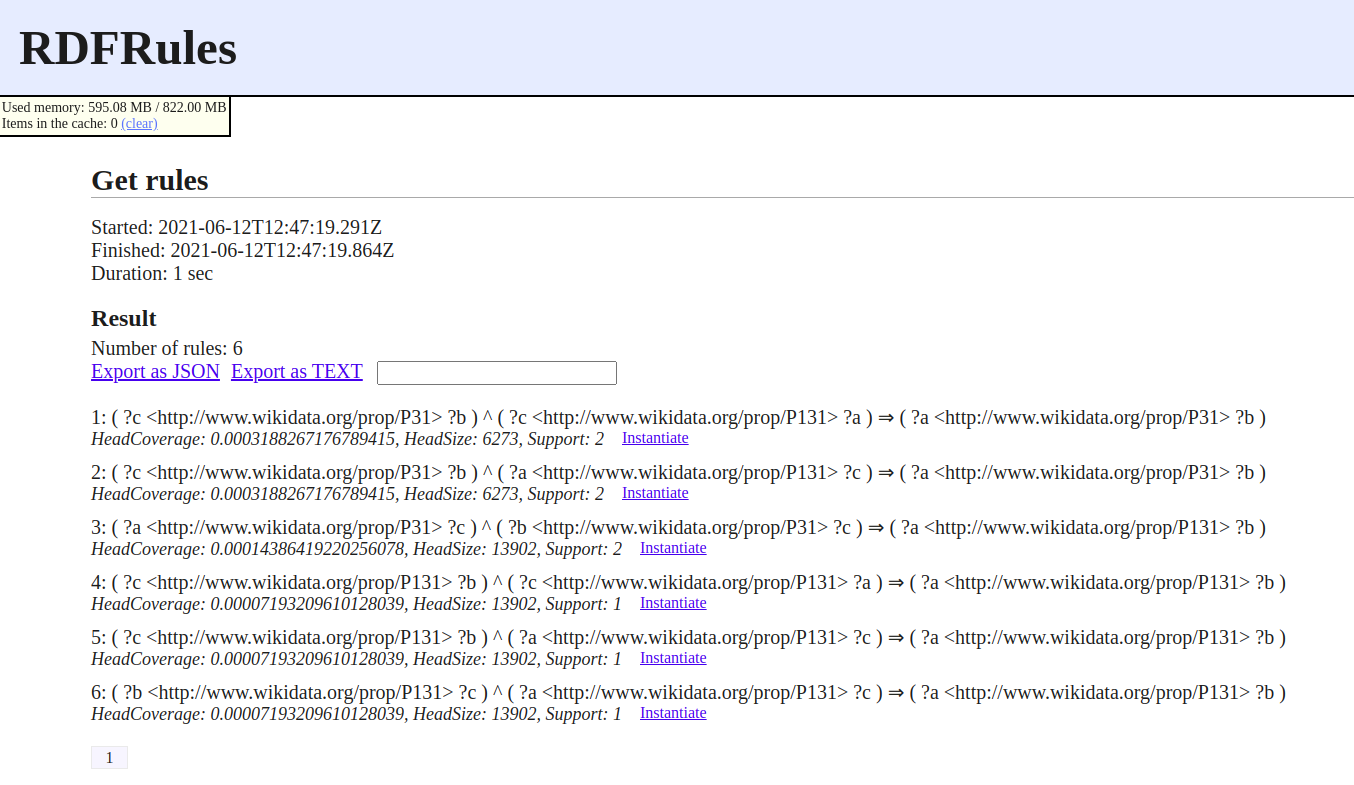
\includegraphics[width=0.8\textwidth]{img/gui-getrules.png}
\caption{RDFRules web browser interface}
\label{rdfrulesgui}
\end{figure}

\section{Data Structures}

The framework's core revolves around four main data structures: \textit{RDFGraph} and \textit{RDFDataset} corresponding to the input data, \textit{Index} wrapping the set of indeces the input data is transformed into and \textit{RuleSet} containing rules generated by the algorithm. These structures are transformed into each other in the stated order during the mining process by applying various operations on them. Inspired by the Apache Spark RDD\footnote{\href{https://spark.apache.org/docs/latest/rdd-programming-guide.html\#resilient-distributed-datasets-rdds}{https://spark.apache.org/docs/latest/rdd-programming-guide.html\#resilient-distributed-datasets-rdds}} the operations are categorized into \textit{transformations} and \textit{actions}. All transformations are \textit{lazy} operations meaning they are not performed right after the API call but only when an action operation is called which is dependent on them.

Each transformation method called on an instance of the data structures returns either a modified version of the same instance or the instance transform into a further data structure but the instance which the method was called on does not change i.e. the objects of the framework are immutable and the whole workflow with the core API lies in chaining those methods. Multiple calls of an action operation with different input parameters would result in repetitive performance of the defined transformations so each data structure has a \textit{cache} method that enables preserving the result of the transformations in memory or on the disk so that they have to be performed only once.

\begin{figure}[h]
\centering
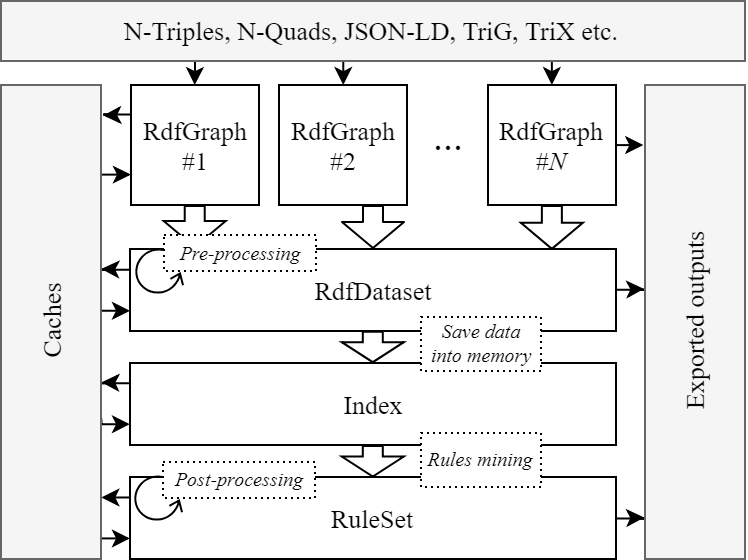
\includegraphics[width=0.6\textwidth]{img/rdfrules-abstractions.png}
\caption{Relations between the RDFRules data structures (Source: \cite{Zeman2018})}
\label{rdfrulesdatastructures}
\end{figure}

%\subsection{RDFGraph and RDFDataset}

An RDFGraph instance corresponds to a set of triples. It is created either from stream of triples or from a file containing a supported RDF serialization (N-Triples, N-Quads, JSON-LD, TriG, Turtle etc.) and optionally can be assigned a graph IRI. RDFDataset can either be created from one or multiple instances of RDFGraph or directly from a file if the input format contains a set of quads so the RDFDataset corresponds to a set of quads. Both RDFGraph and RDFDataset allow filtering, slicing or modifying the data at the level of individual triples/quads. It is possible to merge two instances of RDFGraph, two instances of RDFDataset and to merge an instance of RDFDataset and RDFGraph which results in a new instance of RDFDataset.

Both have a \textit{discretize} method that facades into the EasyMiner-Discretization\footnote{\href{https://github.com/KIZI/EasyMiner-Discretization}{https://github.com/KIZI/EasyMiner-Discretization}} library. It takes a parameter specifying the kind of discretization (\textit{discretization task}) and a parameter in a form of a function that specififies which triples are to be processed. It allows to create a defined number of equidistant and equifrequent intervals or to create equifrequent intervals with a defined minimum frequency (\textit{equisize} discretization task).

%\subsection{Index}

The RDFDataset instance is transformed to an instance of Index on which the rules can be mined with. During this transformation, each resource and literal is assigned a unique number which reprents it in the created indeces. The mining itself, which is triggered by a \textit{mine} method is controlled by defined \textit{pruning thresholds} (pruning during the rule refinement), rule patterns and \textit{constraints}. The available pruning thresholds are minimal head size, minimal head coverage, minimal support, maximum rule length and \textit{timeout} (a time period after which the mining is stopped and so far found rules are returned) in minutes. It also implements the TopK pruning threshold mentioned in \cite{Zeman2020} although only for the head coverage. It does not allow pruning the rules based on minimum confidence as the AMIE+ implementation of Galárraga et al. does. The constraints can specify general characteristics of the rules that can be returned e.g. disallowing duplicit predicates or any constant in the rules.

%\subsection{RuleSet}

The rules are returned by the \textit{mine} method as an instance of RuleSet. Each rule in the set basic measures such as support, head size etc. and other \textit{computationaly expensive} measures such as confidence (PCA or a standard confidence) can be calculated optionally. The rules in the set can be filtered and sorted by those measures. Pruning and clustering can be performed on the set. The algorithm used for clustering is DBScan which takes parameters of minimum size of a cluster, minimum similarity of rules in the same cluster and the weights on the similarity features (whether the clustering should be more based on the rule contents of measures). The rules can be exported into a text file as a human-readable text or in JSON format. Since the mining algorithm and the RuleSet structure do not work with IRIs and literals directly but with their IDs assigned during the creation of indeces, when the rule set is cached into a file, the appropriate instance of Index is needed to restore the rule set, so that the IDs from which the rules consist can be mapped to their IRIs and literals (the rules can be \textit{resolved}).

\begin{lstlisting}[language = scala, caption={An example of a rule mining workflow with RDFRules Scala API (Source: \cite{Zeman2018})}, label={scalascript},captionpos=b, escapeinside={(*@}{@*)}]
Dataset("yago.tsv")
    .filter(!_.triple.predicate.hasSameUriAs("participatedIn"))
    .discretize(DiscretizationTask.Equifrequency(3))
    (_.triple.predicate.hasSameUriAs("hasNumberOfPeople"))
    .mine(Amie()
    .addConstraint(RuleConstraint.WithInstances(true))
    .addPattern(AtomPattern(predicate = Uri("hasNumberOfPeople")) =>: None)
    .addPattern(AtomPattern(predicate = Uri("hasNumberOfPeople"))))
    .computePcaConfidence(0.5)
    .sorted
    .export("rules.json")
\end{lstlisting}

\chapter{Leveraging a Combination of OLAP Cubes and Knowledge Graphs}

OLAP analysis and graphical visualisation suggest itself as natural ways of analyzing statistical linked data. Section \ref{dcv} describes how the statistical data can be represented as RDF using the Data Cube Vocabulary. The effort of anylyzing the statistical RDF data is focused on making use of the \textit{open} rather than \textit{linked} nature of Linked Open Data. Available RDF data is extracted as is and either loaded into an OLAP system  and treated as any other OLAP data \cite{Kämpgen2011} or it is analyzed by SPARQL queries.\cite{Capadisli2013} 

In \cite{Chudan2015} the application of GUHA \cite{Rauch2017} association rules for mining over the aggregated data was suggested as a complement to the standard OLAP analysis. The aggregated observations are treated as individual transactions in tabular data. The mined rules describe strong relations in the cube and can serve as a guide unusual trends that would be otherwise hard to find by manually browsing the OLAP cube.

The following text builds on the idea that some trends in OLAP cube can be expressed in as association rules and elaborates the possibilities of mining association rules by the AMIE algorithm over aggregated data in a form of a data cube. The AMIE algorithm mines rules directly over RDF data which can therefore be enriched by another relations describing the cube's dimension values extractable from other LOD sources so that the \textit{linked} nature of LOD is exploited as well.

\section{Mining from RDF representation of Data Cube}

We are going to aim to mine association rules that describe how a certain measure's values are determined by values of one or more dimensions meaning that the observations of the examined cube corresponding to fixed values of some dimensions (slicing and dicing) tend to contain a measure values with a certain characteristic. Those rules are a subject to the language bias described in \ref{languagebias}. The antecedent of the rule would basicaly specify a certain slice (a subset of observations) of the examined cube in which the measured values deviate from the whole and the consequent of the rule would describe the nature of this deviation.

\subsection{Rules's Bias}

Such a rule (the predicted characteristic of the subset of observations) has to be deducible by the algorithm so its head atom has to be \textit{instantiatable} by triples contained in the examined data set so the head's predicate will be one of the cube's measure, the head's subject will be a variable representing observations for which the rule's antecedent is valid and the head's object will be a specific constant of a discrete measure's value, that is predicted to be associated with all the observations that satisfy the antecedent. For example imagine a very small data cube which arose from a survey on the life satisfaction among men and women in several european countries. In each country a male and a female responsdent was asked to rank their life satisfaction either as \textit{low}, \textit{moderate} or \textit{high}. So the resulting data cube contains two dimensions of \textit{sex} and \textit{country} and a single measure of life satisfaction. Each respondent in the survey corresponds to one observation. 

\begin{table}[h]
\centering
\begin{tabular}{l|lllll}
    & France & Germany & Poland & Slovakia & Austria  \\ 
\hline
Men   & moderate     & high       & moderate      & high        & high        \\
Women & low      & moderate       & high      & low        & low       
\end{tabular}
\end{table}


Based on the results of the survey in the table above we could determine that men accross the countries tend to a high life satisfaction. This fact can be expressed as an association rule that is deducible by the AMIE algorithm.

$$ 
(?o\hspace{0.4em}sex\hspace{0.4em}Male) \Rightarrow (?o\hspace{0.4em}lifeSatisfaction\hspace{0.4em}High) 
$$

We can calculate measures of significance of this rule from the values in the table. Since the object in the rule's head is a constant, the support of the rule corresponds only to the distinct observations that belong to men and have the correct measure value, i.e. \numprint{3}. The head coverage is calculated as support divided by the number of distinct triples with the head's predicate, which is equivalent to the number of distinct observations in the cube (in this example $3 \div 10 =0.\overline{3}$) which \textbf{would be constant for all found rules} so the head coverage does not convey any new information than the support measure when minig such rules from data cubes. 

More interesting is an expression of the prediction's quality. That lead us to the measures of confidence. The standard confidence of the rules would be deducted from the ratio of men that said that they are highly satisfied with their life on all men that participated in the survey. If we assume that all observations are assigned the same number of measures, then the PCA confidence is equivalent to the standard confidence, because all observations satisfying the rule's body would be assigned any constant of the measure appearing in the rule's head. The confidence of the rule above equal to $3 \div 5 = 0.\overline{6}$.

If the cube has more than one measure, one of the measures can be used in the rule's body to further specify the subset of the observations. Let's extend the survey by another question. The respondents also had to rank their salary as either \textit{low}, \textit{decent} or \textit{high}.

\begin{table}[h]
\centering
\begin{tabular}{ll|lllll}
                                 &       & France   & Germany  & Poland   & Slovakia & Austria  \\ 
\hline
\multirow{2}{*}{lifeExpectation} & Men   & moderate & high     & moderate & high     & high     \\
                                     & Women & low      & moderate & high     & low      & low      \\ 
\hline
\multirow{2}{*}{salary}          & Men   & low      & decent   & low      & decent   & decent     \\
                                     & Women & low      & high     & decent   & low      & decent  
\end{tabular}
\end{table}

Now if the rule's body contains a new atom demanding a certain value of the new measure for the observations:

$$ 
(?o\hspace{0.4em}sex\hspace{0.4em}Male) \land (?o\hspace{0.4em}salary\hspace{0.4em}Decent)  \Rightarrow (?o\hspace{0.4em}lifeSatisfaction\hspace{0.4em}High) 
$$

The value of support does not change. Now there are only \numprint{3} observations valid for the rule's body (Men of Germany, Slovakia and Austria) and all those observations are valid for the rule's head as well so the confidence of this rule is equal to \numprint{1}.

\subsection{Commensurability}

In the previous example, the measured values were discrete but data cube usually contain continuos numerical values on which aggregation operations (sum average etc.) are possible. In order to ensure, that the rules can achieve a reasonable support, the numerical values have to be discretized (see \ref{numericalattributes}) and replaced by intervals. But one cannost simply discretize all measure's values at once. The dimension values can be structured into a hierarchy so the measures belonging to dimension values of different levels in the hierarchy are not comparable.\cite{Chudan2015} Irrespective to a chosen discretization approach, it is inadmissible to discretize values belonging to different disproportionate contexts.

One way to solve this to dice a cube having disproportionate dimension values into a set of smaller subcubes, in which the dimension values belong to the same level of a concept hierarchy. Measured values can be then discretized into intervals in each subcube separately. Number of subcubes that the main cube has to be divided into depends on the number dimensions and the number of levels in each dimension’s hierarchies. It assumes that the information about the structure of the hierarchy is available. The rules would be mined either separately on each subcube or for each observation a triple with the assignment of the observation to its subcube would have to be added into to the data set and this assignment would have to be stated in the body of the rules.

An alternative to this proposed in \cite{Koukal2017} could be to cluster the values of each measure in the whole cube by the k-means algorithm a then to create equifrequent intervals inside those clusters. This would be useful when there is a significant difference in measurements belonging to the same level of hierarchy for a dimension. \cite{Koukal2017} gives an example of sales distribution among different products in a hypermarket. The number of sales of bakery will be incomparable to number of sales of electric razors. In the context of the AMIE algorithm, the assignment of each observation to each measure's cluster would have to be added to the data set and then expressed in the rule's body, otherwise also the observations belonging to different clusters would be considered counterexamples and the confidence would not be computed properly. One disadvatage of this approach is that there is no clear interpretation of the generated subcubes. Their observations can belong to different levels of the concept hierarchy in a dimension. Unlike with the previous approach where a generated subcube could be described as for example \textit{population in districts by age category}.


The following example explains the first approach. Adam and Beatrice work as food delivery persons. Data about the amount of their delivered orders in 2020 is entered in a data cube with two dimensions of the person delivering and the time interval to which the number of delivered orders relates. The length of time intervals varies. They are either whole weeks or whole months.

\begin{table}[h]
\centering
\begin{tabular}{l|llllll}
         & 1st Week & 2nd Week & 3rd Week & January & February & March  \\ 
\hline
Adam     & 50               & 55               & 40               & 150     & 250      & 200    \\
Beatrice & 30               & 40               & 20               & 100     & 120      & 130   
\end{tabular}
\end{table}

The values belonging to weeks are not comparable with the values belonging to months. The cube will be sliced into two cubes, with one containing the observations of week and the second with observations of months. Values will be then discretized in both cubes separately. For the sake of simplicity, the values will be discretized into two equifrequent intervals.

\begin{table}[h]
\centering
\begin{tabular}{l|llllll}
             & 1st Week & 2nd Week & 3rd Week & January  & February & March     \\ 
\hline
Adam     & ef2/2\_1 & ef2/2\_1 & ef1/2\_1 & ef2/2\_2 & ef2/2\_2 & ef2/2\_2  \\
Beatrice & ef1/2\_1 & ef1/2\_1 & ef1/2\_1 & ef1/2\_2 & ef1/2\_2 & ef1/2\_2 
\end{tabular}
\end{table}

Let's have a rule stating that Beatrice's weekly delivered orders \textit{are low} (in the lower of the two equifrequent intervals). The assignment of the valid observations to the correct subcube has to be part of the body so that the Beatrice's montly order values are not considered counterexamples. In Data Cube Vocabulary, this assignment is provided by the $qb:dataSet$ property.

$$ 
(?o\hspace{0.4em}person\hspace{0.4em}Beatrice) \land (?o\hspace{0.4em}qb:dataSet\hspace{0.4em}Week)  \Rightarrow (?o\hspace{0.4em}orders\hspace{0.4em}ef1/2\_1) 
$$

The question is to how many intervals the measures should be discretized into. If creating too many intervals, more specific rules should be found but they happen to have a lower support. When performing the equifrequent discretization, coarser rules are found for lower number of intervals. To avoid guessing which discretization parameters suit best the data, multiple discretizations can be performed with different parameters for various discretization algorithms. As it was already mentioned, the preprocessed cube should to be cut into subcubes with commensurable observations, measures in theses subcube have to be discretized separately and only after that the triples can be merged and performed the mining tasks on.

\begin{figure}[h]
\begin{lstlisting}[language = turtle, caption={Observations example}, label={obsexample},captionpos=b escapeinside={(*@}{@*)}]
@prefix qb: <http://purl.org/linked-data/cube#> .

<o1> qb:dataSet <original-dataset> ;
    <dimension1> <dimension1value1> ; <dimension2> <dimension2value1> ;
    <measure1> 25000 ;
    <measure2> 3 .
    
<o2> qb:dataSet <original-dataset> ;
    <dimension1> <dimension1value2> ; <dimension2> <dimension2value2> ;
    <measure1> 10000 ;
    <measure2> 10 .
\end{lstlisting}
\end{figure}

That means that the number of overall \textit{measurements} multiplies by the number of distinct discretizations. A situation has to be avoided, when the instantiations of variable representing observations are involving observations not only from various subcubes but also those observations are assigned measurements from dijunct sets of intervals (distinct discretizations). The result of a approach (let's call it style $A$) to solve this problem on the sample data in \ref{obsexample} is shown in \ref{discsample}.

\begin{figure}[h]
\begin{lstlisting}[language = turtle, caption={Discretization example}, label={discsample},captionpos=b escapeinside={(*@}{@*)}]
@prefix qb: <http://purl.org/linked-data/cube#> .
            
<o1> qb:dataSet <subcube1> ;
    <dimension1> <dimension1value1> ; <dimension2> <dimension2value1> ;
    <measure1> <subcube1_ef3_measure1_3>, <subcube1_ef10_measure1_2> ;
    <measure2> <subcube1_ef3_measure2_2>, <subcube1_ef10_measure2_1> .
   
<o2> qb:dataSet <subcube2> ;
    <dimension1> <dimension1value2> ; <dimension2> <dimension2value2> ;
    <measure1> <subcube2_ef3_measure1_3> , <subcube2_ef10_measure1_2> ;
    <measure2> <subcube2_ef3_measure2_1> ,<subcube2_ef10_measure2_1> .
\end{lstlisting}
\end{figure}

Each application of a discretization algorithm will create a new measurement triple for each measure and observation with an object of the assigned interval based on the discretization algorithm and the parameter. The objects in triples assigning the observations to a data set will be changed to point to the particular subcube. In the example two discretizations for each measure were performed on the two observations. In the example the same pair of discretizations were performed on the two distinct measures, but that does not have to be so. Assigning multiple triples of the same measure is fine as far as the measure is differently discretized.

In each rule it has to be ensured, that the set of observations is limited to a certain subcube. For each cube in a rule the body of a rule has to contain an atom of a pattern $(?o\hspace{0.4em}qb:dataSet\hspace{0.4em}AnyConstant)$. The discretized subcubes can be either be performed mining tasks on separately or they could remain as a singe data set. The second option is less demanding. A single index is created from which a single rule set is generated. It distorts the lift measure though, because it increases the denominator of the head confidence. To show the effect let's return to the example of Adam and Beatrice and let's compute the head confidence\footnote{We calculate on the head confidence as the denominator of the lift formula since the formula's numerator (confidence) does not change.} of the rule first for the case when the subcubes\footnote{That means one subcube of the weekly order amounts and one subcube of the monthly order amounts.} are mined on seperately. The examined rules would be contained in the rule set generated from mining the \textit{weekly} subcube.

$$hconf(\vec{B} \Rightarrow H) = \frac{\# s: \exists \langle s,p,o\rangle \prec (?a\hspace{0.4em}p\hspace{0.4em}C) }{\# s: \exists \langle s,p,o\rangle \prec (?a\hspace{0.4em}p\hspace{0.4em}?b)} = \frac{3}{6} = \frac{1}{2}$$

If we mined over the whole cube, the head confidence's denominator would consider all observations in the cube.

$$hconf(\vec{B} \Rightarrow H) = \frac{\# s: \exists \langle s,p,o\rangle \prec (?a\hspace{0.4em}p\hspace{0.4em}C) }{\# s: \exists \langle s,p,o\rangle \prec (?a\hspace{0.4em}p\hspace{0.4em}?b)} = \frac{3}{12} = \frac{1}{4}$$

The head coverage is disorted both by mining over multiple subcubes and by performing multiple discretization of the same measure, because its denominator as the number of triples with the head's predicate, named head size. Each performed discretization over a measure increases this number by the number of observations and so does the inclusion of triples with observations not compatible with a rule. Let's compute the head size of the above mentioned rule when mined only from the \textit{weekly} subcube.

$$
hsize(\vec{B} \Rightarrow (s\hspace{0.4em}p\hspace{0.4em}o)) = \# \langle s,p,o\rangle \in KG: \langle s,p,o\rangle \prec (?a\hspace{0.4em}p\hspace{0.4em}?b) = 6 
$$

Since there are only 6 observations in the whole mined data set. Let's perform a second discretization over Adam's and Beatrice's data cube and also mine over the whole cube. 

\begin{table}[h]
\centering
\begin{tabular}{l|llllll}
                          & 1st Week & 2nd Week & 3rd Week & January  & February & March     \\ 
\hline
\multirow{2}{*}{Adam}     & ef2/2\_1 & ef2/2\_1 & ef1/2\_1 & ef2/2\_2 & ef2/2\_2 & ef2/2\_2  \\
                          & ef3/3\_1 & ef3/3\_1 & ef2/3\_1 & ef2/3\_2 & ef3/3\_2 & ef3/3\_2  \\
\multirow{2}{*}{Beatrice} & ef1/2\_1 & ef1/2\_1 & ef1/2\_1 & ef1/2\_2 & ef1/2\_2 & ef1/2\_2  \\
                          & ef1/3\_1 & ef2/3\_1 & ef1/3\_1 & ef1/3\_2 & ef1/3\_2 & ef2/3\_2 
\end{tabular}
\end{table}

Now the head size will be higher because all 12 observations are considered plus their count is multiplied by the number of performed observations.

$$
hsize(\vec{B} \Rightarrow (s\hspace{0.4em}p\hspace{0.4em}o)) = \# \langle s,p,o\rangle \in KG: \langle s,p,o\rangle \prec (?a\hspace{0.4em}p\hspace{0.4em}?b) = 12 * 2 = 24
$$

A different way of structuring the discretized measures (let's call it style $B$) within the observations would remove both distortions while also permitting to mine over the whole original cube. Each performed discretization would introduce a new derived measure whose name could be chosen as the name of the original measure suffixed by type of discretization with its parameters and the observation's subcube.

\begin{figure}[h]
\begin{lstlisting}[language = turtle, caption={Discretization example 2}, label={discsample},captionpos=b escapeinside={(*@}{@*)}]
@prefix qb: <http://purl.org/linked-data/cube#> .
                
<o1> qb:dataSet <subcube1> ;
    <dimension1> <dimension1value1> ; <dimension2> <dimension2value1> ;
    <subcube1_ef3_measure1> <subcube1_ef3_measure1_3> ;
    <subcube1_ef10_measure1> <subcube1_ef10_measure1_2> ;
    <subcube1_ef3_measure2> <subcube1_ef3_measure2_2> ; 
    <subcube1_ef10_measure2> <subcube1_ef10_measure2_1> .
       
<o2> qb:dataSet <subcube2> ;
    <dimension1> <dimension1value2> ; <dimension2> <dimension2value2> ;
    <subcube2_ef3_measure1> <subcube2_ef3_measure1_3> ;
    <subcube2_ef10_measure1> <subcube2_ef10_measure1_2> ;
    <subcube2_ef3_measure2> <subcube2_ef3_measure2_1> ;
    <subcube2_ef10_measure2> <subcube2_ef10_measure2_1> .
\end{lstlisting}
\end{figure}

The head coverage of a rule generated from such data can be then interpreted as the ratio of the rule's support and the number of appropriate observations regardless of whether the whole cube is mined at once or the subcubes are mined separately because the predicate of the rule will be anchored both to the appropriate subcube and to a single performed discretization. This would however disadvantage finer discretizations because they would tend to have lower and support while the head size would be constant accross all rules with associated with the same subcube and the same original measure.

The support of a rule is affected by the number of observations of the subcube to which the rule is anchored. The rules generated for a bigger subcube will tend to have a higher support compared to rules from a smaller subcubes because there will be more observations that can meet the condition of the rule's body. But this effect is cancelled out in the head coverage because with more observations its numerator (support) grows but its denominator grows as well. So for a cube constisting of a high number of subcubes it can be suggested to use the style B of expressing the discretized measures and mined the cube at once with a defined head coverage parameter. A low number of subcubes could be mined separately with a custom minimum support threshold defined for each subcube to tweak each subcube's rule set. And since the separate mining of each subcube solves the lift distortion by itself and a minimum support threshold would be used instead of a minimum head coverage, the measure expression style $A$ could be used because it's propably easier to perform.

\begin{table}[h]
\centering
\begin{tabular}{l|ll}
                           & style A                       & style B                  \\ 
\hline
mining the whole cube      &                               & high no. of subcubes  \\
mining subcubes separately & manageable no. of subcubes &                         
\end{tabular}
\end{table}

\section{Appending RDF Data to the Data Cubes}

So far the showed rules specified the subset of observations only by exactly one value for a dimension, just as e.g. the Apriori algorithm's rules contain only one category for each atribute. Slicing the subset of observations just by one value per dimension would yield just a contrained set of rules. The language bias of the AMIE algorithm does not allow a collection (disjunction) of values in the atom's object. It can be either a constant or a variable. But a variable can appear in another atom in which it is attributed a \textit{property}. That way the variable acts as a collection of entities sharing this property.

If the dimension values represent a real-world entities such as geographical areas, persons, organizations etc., such properties can be found in the form of RDF triples published in public knowledge graphs. Those triples can enter the algorithm together with the triples describing the data cube. Let's continue with the example of Adam and Beatrice. Table below shows a simple data cube containing the numbers of their daily delivered orders from July 14th to 17th. Each cells contains the original value of daily orders plus its interval after the equifrequent discretization into four intervals.

\begin{table}[h]
\centering
\begin{tabular}{l|llll}
Orders                    & 07-14 & 07-15 & 07-16 & 07-17  \\ 
\hline
\multirow{2}{*}{Adam}     & 10    & 7     & 6     & 0      \\
                         & ef4/4 & ef3/4 & ef2/4 & ef1/4  \\
\multirow{2}{*}{Beatrice} & 9     & 0     & 8     & 4      \\
                          & ef4/4 & ef1/4 & ef3/4 & ef2/4 
\end{tabular}
\end{table}

Both also publish their personal information as RDF with the \textit{FOAF} Vocabulary\footnote{\href{http://www.foaf-project.org/}{http://www.foaf-project.org/}} on their blogs. The listing \ref{foafexample} shows a deluge of both person's information.

\begin{figure}[h]
\begin{lstlisting}[language = turtle, caption={RDF data published on Adam's and Beatrice's personal blogs}, label={foafexample},captionpos=b escapeinside={(*@}{@*)}]
@prefix foaf: <http://xmlns.com/foaf/0.1/> .

<http://adamsmith.xyz/#me>
    a foaf:Person ;
    foaf:name "Adam Smith" ;
    foaf:givenname "Adam" ;
    foaf:family_name "Smith" ;
    foaf:birthday "07-17"^^xsd:string ;
    foaf:homepage <http://www.adamsmith.xyz> .
      
<http://beatricet.com/#me>
    a foaf:Person ;
    foaf:name "Beatrice Taylor" ;
    foaf:givenname "Beatrice" ;
    foaf:family_name "Taylor" ;
    foaf:birthday "07-15"^^xsd:string ;
    foaf:homepage <http://www.beatricet.com> .
\end{lstlisting}
\end{figure}

If this data is merged with the data cube, one of the rules found by AMIE algorithm would be a rule stating that a when a person has a birth day, their number of delivered orders in that day is in the lowest of four equifrequent intervals. For this simple example it could also predict the exact zero. Probably because when someone has a birth day, they have a party with friends or with family and they do not bother with delivering meals.

$$
(?o\hspace{0.4em}day\hspace{0.4em}?b) \land (?p\hspace{0.4em}foaf:birthday\hspace{0.4em}?b)
$$
$$ 
\land (?o\hspace{0.4em}person\hspace{0.4em}?p) \land (?o\hspace{0.4em}qb:dataSet\hspace{0.4em}Day)  \Rightarrow (?o\hspace{0.4em}orders\hspace{0.4em}ef1/4) 
$$

This example is simplified in the way that it assumes that the IRIs representing Adam and Beatrice in the data cube are identical to the IRIs they assigned to themselves and also that the data cube uses the same date format as the \textit{FOAF} Vocabulary suggests. Which would not because the cube's dates represent actual days, whereas birth day is just a combination of month and day repeating every year, so this relation would have to be inferred by another triples whose atom would have to be in the rule. The dimension values do not just have to be \textit{described} directly. The rule can contain a \textit{chain} of atoms not instantiated by the cube's triples starting with the dimension value's variable.

Real-world entities or concepts can be assigned multiple identifiers in the LOD environment. In order to the AMIE algorithm to make the right connection between the dimension values and triples from other sources describing them, the identifiers have to either be unified or triples stating their equivalence e.g. with the \textit{owl:sameAs} predicate have to be added into the data set and those connections have to be part of the rules.

\section{Finding Rules Concerning Multiple Cubes}

The same dimension values of a data cube can be present in other data cubes either with the same or a different identifier. For example both a cube containing procurement statistics of a country and a cube containing demography statistics of the country would have a dimension of the reference areas in the country. The measures attributed a dimension value in a data cube can be considered properties describing the dimension value, therefore there is a possibility to use it to specify the subset of observations in an examined cube just as the RDF data from public knowledge graphs. But one has to remember that the measures are given in the context of all dimensions in the cube. 

Let's have a first example of two small data cubes. One contains averages salary statistics by region, year and sex. The second cube contains average pension statistics by region and year.

\begin{table}[h]
\centering
\begin{tabular}{ll|lll|lll}
\multicolumn{2}{l|}{\multirow{2}{*}{Dimensions}} & \multicolumn{3}{c|}{Salaries}                                                   & \multicolumn{3}{c}{Pensions}                                                    \\
\multicolumn{2}{l|}{}                            & \multicolumn{1}{c}{2010} & \multicolumn{1}{c}{2011} & \multicolumn{1}{c|}{2012} & \multicolumn{1}{c}{2010} & \multicolumn{1}{c}{2011} & \multicolumn{1}{c}{2012}  \\ 
\hline
\multirow{2}{*}{Region 1} & Male                 & High                     & High                     & High                      & \multirow{2}{*}{Medium}  & \multirow{2}{*}{High}    & \multirow{2}{*}{High}     \\
                          & Female               & Medium                   & Medium                   & High                     &                          &                          &                           \\
\multirow{2}{*}{Region 1} & Male                 & Low                      & Medium                   & High                      & \multirow{2}{*}{Low}     & \multirow{2}{*}{Low}     & \multirow{2}{*}{Low}      \\
                          & Female               & Low                      & Low                      & Low                       &                          &                          &                          
\end{tabular}
\end{table}

The cubes vary in the number of dimensions but they share the dimensions of region and year. We can imagine this rule generated by AMIE algorithm:

$$
(?o1\hspace{0.4em}qb:dataSet\hspace{0.4em}Salaries) \land (?o1\hspace{0.4em}salary\hspace{0.4em}High) \land (?o1\hspace{0.4em}sex\hspace{0.4em}Male)
$$
$$
\land (?o2\hspace{0.4em}region\hspace{0.4em}?r) \land (?o1\hspace{0.4em}region\hspace{0.4em}?r) \land (?o1\hspace{0.4em}year\hspace{0.4em}?y)
$$
$$
\land (?o2\hspace{0.4em}year\hspace{0.4em}?y) \land (?o2\hspace{0.4em}qb:dataSet\hspace{0.4em}Pensions) \Rightarrow (?o2\hspace{0.4em}pension\hspace{0.4em}High)
$$

which states that if there is an observation in the \textit{Salaries} cube assigned to Males and to some region and year and this observation's measure for average salary reads \textit{High}, then all observations from the \textit{Pensions} cube assigned to the same region and year have the average pension measure value of \textit{High}. This can be paraphrased as: \textit{People in regions where men have high salaries have high pensions.} For each observation from the \textit{Salaries} cube that satisfies the rule's there is exactly one observation from the \textit{Pensions} cube that does as well given that the ranges of the region and year dimensions in the \textit{Salaries} cube are subsets or identical sets of the the same dimensions in the \textit{Pensions} cube. 

Let's refer to the cubes whose observations are instantiated in the variable that appears in a rule's head as \textit{head cubes} and the cubes whose observation are instantiated in the variable that appears only in a rule's body as \textit{body cubes}. There can be one or more body cube and exactly one head cube in a rule. The \textit{Salaries} cube in the rule above is a body cube and the \textit{Pensions} cube is a head cube. If a cube's dimension appears in the rule, let's refer to the cube's dimension as \textit{closed} for the rule and it does not appear in the rule, let's refer to the dimension as \textit{open}. All the \textit{Salaries} cube's dimension in the rule above are closed and so are all the dimensions of the \textit{Pensions} cube.

If one or more dimensions of a body cube are open in a rule, then the interpretation of the becomes complicated. The rule below was mined from the same cubes with the same structure, but the \textit{Salaries} cube has open dimension (sex) in the rule.

$$
(?o1\hspace{0.4em}qb:dataSet\hspace{0.4em}Salaries) \land (?o1\hspace{0.4em}salary\hspace{0.4em}High) \land (?o2\hspace{0.4em}region\hspace{0.4em}?r)
$$
$$
\land (?o1\hspace{0.4em}region\hspace{0.4em}?r) \land (?o1\hspace{0.4em}year\hspace{0.4em}?y) \land (?o2\hspace{0.4em}year\hspace{0.4em}?y)
$$
$$
\land (?o2\hspace{0.4em}qb:dataSet\hspace{0.4em}Pensions) \Rightarrow (?o2\hspace{0.4em}pension\hspace{0.4em}High)
$$

This rule states that if either men or women have high salary in a region then people have high pensions in the region. If there is an open dimension of a body cube, it adds an \textit{or} statement into the rule's interpretation for each distinct value of the open dimension. Therefore open dimensions in the body cubes should be avoided unless the number of distinct values of an open dimension is very low. Following example shows how the interpretability of a rule is affected when all body cubes have only closed dimensions but one head cube's dimension is open. The cubes have now a different structure.

\begin{table}[h]
\centering
\begin{tabular}{ll|lll|lll}
\multicolumn{2}{l|}{\multirow{2}{*}{Dimensions}} & \multicolumn{3}{c|}{Salaries}                                                   & \multicolumn{3}{c}{Pensions}                                                    \\
\multicolumn{2}{l|}{}                            & \multicolumn{1}{c}{2010} & \multicolumn{1}{c}{2011} & \multicolumn{1}{c|}{2012} & \multicolumn{1}{c}{2010} & \multicolumn{1}{c}{2011} & \multicolumn{1}{c}{2012}  \\ 
\hline
\multirow{2}{*}{Region 1} & Male                 & \multirow{2}{*}{Medium}  & \multirow{2}{*}{High}    & \multirow{2}{*}{High}     & Medium                   & High                     & High                      \\
                          & Female               &                          &                          &                           & Medium                   & Medium                   & Medium                    \\
\multirow{2}{*}{Region 1} & Male                 & \multirow{2}{*}{Low}     & \multirow{2}{*}{Medium}  & \multirow{2}{*}{High}     & Low                      & Low                      & Low                       \\
                          & Female               &                          &                          &                           & Medium                   & Low                      & Low                      
\end{tabular}
\end{table}

The \textit{Salaries} cube has the dimensions of region and year and the \textit{Pensions} cube has the dimensions of region, year and sex. In the rule below the head cube has one open dimension of sex. In the context of the cubes' structure the rule would be interpreted as \textit{if in any year the salaries in a region are high then the male pensions and female pensions are high in this region that year}. For each \dots

% todo for each ...

\begin{minipage}{\textwidth}
$$
(?o1\hspace{0.4em}qb:dataSet\hspace{0.4em}Salaries) \land (?o1\hspace{0.4em}salary\hspace{0.4em}High) \land (?o2\hspace{0.4em}region\hspace{0.4em}?r)
$$
$$
\land (?o1\hspace{0.4em}region\hspace{0.4em}?r) \land (?o1\hspace{0.4em}year\hspace{0.4em}?y) \land (?o2\hspace{0.4em}year\hspace{0.4em}?y)
$$
$$
\land (?o2\hspace{0.4em}qb:dataSet\hspace{0.4em}Pensions) \Rightarrow (?o2\hspace{0.4em}pension\hspace{0.4em}High)
$$
\end{minipage}

If there is an open dimension of the head cube, it adds an \textit{and} statement into the rule's interpretation for each distinct value of the open dimension.

% že to tolik nevadí??
% consistent over

\section{Note to the Rule's Atom Order}

% could be more human readable if the 

% tyto výskyty v jiných kostkách ; measures prisouzene tem dimension values se dají povazovat za jejich properties a se dají taky použít taky pro specifikaci subsetu observation in an examined cube



% ten subset se dá omezit i informacemi v jiné kostce

% linking musí fungovat mezi kostkama
\chapter{Experiment}

% TODO nějaký úvod, že ukazuju, jak je možné kombinovat OLAP a KG, co jsem použil za technologie, proč to dělám REPL

This section describes an experiment of mining associtation rules from RDF data compiled of statistical data structured by the Data Cube Vocabulary and facts pulled from the Wikidata data set that was performed as an practical part of this work. The statistical data come from two sources. The first one is the Czech Social Security Administration and the second one is the Czech Statistical Office. Analysis was performed using the Scala API of the reference implementation of the RDFRules algorithm. The following sectins describe how the available data had to be preprocced to give reasonable results in combination with KG data. The preprocessing was perfomed partly by the implementation's API itself, partly by performing SPARQL queries over the data. The described method can be taken inspiration from when performing similar analysis ie. association rule mining task over the multidimensional data merged with loosely structured graph data. 

\section{Czech Social Security Administration}

Czech Social Security Administration (CSSA) is a czech public administration organtisation responsible for collecting social security premiums and contributions to the state employment policy. Since 2015 the organization publishes its statistical yearbook datasets and other (vocabularies, code lists and datasets containing data concerning the internal operation of the organization) in the form LOD and became of the first czech public institutions to do so. The yearbook statistical data sets are modelled using Data Cube Vocabulary. Their dimension values are represented by the SKOS vocabulary. The organization has published 73 datasets so far. All these datasets are downloadable as dumps\footnote{\href{http://data.cssz.cz/web/otevrena-data/katalog-otevrenych-dat}{http://data.cssz.cz/web/otevrena-data/katalog-otevrenych-dat}} or accesible througth a SPARQL endpoint\footnote{\href{http://data.cssz.cz/web/otevrena-data/sparql-query-editor/}{http://data.cssz.cz/web/otevrena-data/sparql-query-editor/}}. The CSSA's URI are dereferenceable.

% project vše
% že tam jsou i CSV data a pro každý data set je stránka s popisem

The largest of the data cubes published is \verb|cssad:duchodci-v-cr-krajich-okresech|\footnote{https://data.cssz.cz/resource/dataset/duchodci-v-cr-krajich-okresech}. From now on it will be denoted as CSSA1. It contains \numprint{368118} observations structured spread over four dimensions: reference area\footnote{https://data.cssz.cz/ontology/dimension/refArea}, reference period\footnote{https://data.cssz.cz/ontology/dimension/refPeriod}, sex\footnote{https://data.cssz.cz/ontology/dimension/pohlavi} and pension kind\footnote{https://data.cssz.cz/ontology/dimension/druh-duchodu}. Observations are assigned three measures: the average amount of pension\footnote{https://data.cssz.cz/ontology/measure/prumerna-vyse-duchodu-v-kc}, the average age\footnote{https://data.cssz.cz/ontology/measure/prumerny-vek} and the number of persons\footnote{https://data.cssz.cz/ontology/measure/pocet-duchodcu}. Each observation is assigned only one measure.

% Example of an observation

% kolik je čeho, dimenze ref area, že jsou v code listu, že to jsou proxy entities

% pension kinds pension kinds defined by the Czech legislation

% The code list of regions is based on one of Czech Republic’s base registries, It does not have a LOD interface yet, so we create it as part of OpenData.cz activities.

% The State Administration of Land Surveying and Cadastre (SALSC) 15 runs the Registry of Territorial Identification, Addresses and Real Estate (RTIAR).

% It is one of the base registries in the Czech Republic and therefore, all public administration systems have to link to it

% This makes RTIAR an important link target for the Czech LOD since it may interlink datasets of different publishers through their shared administrative units or buildings.

% Nevertheless, there is an unofficial transformation by the Opendata.cz initiative 16

% Multiple Czech LOD datasets, such as the CSSA statistics, started to use it as a provisional link target.


% linking can be done simply based on the equality of these codes during data transformation

% Since the RTIAR codes are reference codes by law, it is obligatory for CSSA to have them correct. Therefore, also the resulting links are correct.

% Reference time intervals: The data.gov.uk Time Intervals 20 are reused in many British datasets. It is a service providing a Linked Data resource and extensive description for each time instant and time interval, e.g. http://reference.data.gov.uk/ id/gregorian-year/2012 for the year 2012. Resources from this dataset are also used in examples in the DCV specification and it seemed a natural candidate for reuse in the CSSA statistical data cubes as well.

% proxy entities

%The CSSA data uses proxy entities for reused code lists. This means that instead of using the original code list item IRIs directly as objects in the RDF triples, their proxies, https://data.cssz.cz/resource/reference.data.gov. uk/id/gregorian-year/2012 for example, are used in- stead. The CSSA proxies also contain data important to the CSSA, mainly the labels.

% so that the code list items themselves are dereferenceable to the CSSA domain, and their availability and potential versioning isunder the control of the CSSA itself

% code lists published as an individual data set


\section{Czech Statistical Office}

% TODO data o ČSÚ, něco o ČSÚ, jak vznikla data, dostupné datasety, hodnoty dimenzé, jak se k datům dostat, že URI nejsou dereferencovatelné

\section{Linking}

% linking data sets versus linking dimension values

% denote data sets by nejaka zkratka, treba CSSA1, CZSO2

% cssa regiony jsou proxy entities, ktere byly spojene pres owl:sameAs na stejné entity jako CSU, ale ted sou napojene na nejake jine, ktere nejsou dereferencovatelné

% TODO wikidata -> co tam využiju za dta, jak se k nim dostat, jaké je potřeba předzpracování

% TODO YAGO -> co tam využiju, jak se k datům dostanu, jaké je potřeba předzpracování

% TODO Linking

\section{Mining Tasks}

% TODO samotné bádání

\section{Discussion}
\chapter*{Conclusions}
\addcontentsline{toc}{chapter}{Conclusions}

The goal of this work was to explore the possibilities of enriching RDF data cube with the data from publicly available knowledge graphs and mining rules from this data. Section~\ref{combining} contains a description of steps needed in the data pre-processing phase, a type of rules that can be mined from the data, and how this type affects the interest measures of the RDFRules algorithm based on how the input data is structured. This knowledge was used when performing the experiment described in section \ref{experiment}, which yielded results confirming the validity of the suggested approach, which was also a goal of this work. The RDFRules framework proved to be well suited for this type of experiment, thanks to its native recognition of the $owl:sameAs$ predicates and ability to control the shape of the generated rule with its powerful rule pattern syntax. The source codes of the mining procedures and sets of the found rules are available in a Github repository at \href{https://github.com/nvkp/diploma-thesis-code}{https://github.com/nvkp/diploma-thesis-code}.

The extraction and pre-processing of the data were very time-consuming, but there is a lot of room to automate not only this task. For the dimension values of the examined cubes, automatic \textit{record linkage} \cite{Sheth2013} tools could be used to automate the discovery of relevant triples in other data sources, which the data set can be augmented. Also, a tool can be imagined, that would examine the cubes' dimension value, which would infer the suitable way to cut the cube into the commensurable subcubes based on the hierarchy of the dimension value if they were described with SKOS or any other similar vocabulary, and on the characteristics of the measurements associated with the dimension values. Another tool could aid the post-processing phase by compensating for the interest measures' distortions based on the content of the rules and based on the structure of the cubes. 

Regarding the RDFRules framework core API, as described in \ref{note}, the framework permits a definition of a rule pattern matching rules, that the algorithm cannot generate, which results in zero rules found. A functionality to the framework could be added, that would check for the validity of a rule pattern, and it would either try to repair the rule pattern by rearranging the atom patterns in the rule pattern's body or it would simply provide feedback to the user. Also, the user-friendliness of both the core API and the Web UI would be improved if not only single alphabetical characters moreover, in alphabetical order from the head, are allowed for the names of variables in the rule patterns.

%%% Seznam použité literatury
%%% Bibliography
\printbibliography[title={List of References},heading={bibintoc}]

%%% Přílohy k práci, existují-li. Každá příloha musí být alespoň jednou
%%% odkazována z vlastního textu práce. Přílohy se číslují.
%%% Attachments to thesis, if any. Each attachment must be referenced at 
%%% least once in your own text. The appendices are numbered.
%\part*{\Prilohy}
%\appendix
%\chapter{Queries and Scripts}

% todo scala
\begin{lstlisting}[language = scala, caption={Scala script for creating SPARQL queries for preproccesing the CSSA1 data set}, label={scalascript},captionpos=b, escapeinside={(*@}{@*)}]
import scala.io.Source
import java.io.PrintWriter
import scala.sys.process._
    
val byRegion = """
?observation cssz-dimension:refArea ?refAreaCSSA .
GRAPH <https://data.cssz.cz/resource/dataset/pomocne-ciselniky> {
    ?refAreaCSSA a <https://data.cssz.cz/ontology/ruian/Vusc> .
}
"""
    
val byDistrict = """
?observation cssz-dimension:refArea ?refAreaCSSA .
GRAPH <https://data.cssz.cz/resource/dataset/pomocne-ciselniky> {
    ?refAreaCSSA a ?class .
    FILTER (?class IN (
        <https://data.cssz.cz/ontology/ruian/Okres>,
        <https://data.cssz.cz/ontology/ruian/SpravniObvod>
        )
    )
}
"""
    
val stateTotal = """
?observation cssz-dimension:refArea <https://data.cssz.cz/resource/ruian/staty/1> .
"""
    
val bySex = """
NOT EXISTS {
    ?observation cssz-dimension:pohlavi <https://data.cssz.cz/ontology/sdmx/code/sex-T>
}
"""
    
val bothSexes = """
?observation cssz-dimension:pohlavi <https://data.cssz.cz/ontology/sdmx/code/sex-T> .
"""
    
val template = """
PREFIX qb: <http://purl.org/linked-data/cube#>
PREFIX cssz-dimension: <https://data.cssz.cz/ontology/dimension/>
    
CONSTRUCT {
    ?observation ?p ?o
}
WHERE {
    
    ?observation qb:dataSet <https://data.cssz.cz/resource/dataset/duchodci-v-cr-krajich-okresech> .
    ?observation ?p ?o .
    %s
    ?observation cssz-dimension:druh-duchodu <%s> .
    %s
}
"""
    
val commandTemplate = "../../jena/bin/arq --data \"../../data/pensions-filtered.ttl\" --data \"../../data/pomocne-ciselniky.trig\" --query \"queries/%s.rq\" > \"results/%s.ttl\""
val source = Source.fromFile("pensionkinds.txt")
val lines = source.getLines().toArray
val pw = new PrintWriter(s"script.sh") 
lines.foreach(line => {
        
    val kindName = line.replaceAll("https://data.cssz.cz/resource/pension-kind/","").replaceAll("_2010","")
    val districtTotalQuery = template.format(bothSexes,line,byDistrict)
    val districtTotalFileName = s"pensions-by-district-total-$kindName"
    val districtTotalPw = new PrintWriter(s"queries/$districtTotalFileName.rq")
    districtTotalPw.print(districtTotalQuery)
    districtTotalPw.close()
    pw.println(commandTemplate.format(districtTotalFileName,districtTotalFileName))
    
    val districtBySexQuery = template.format(bySex,line,byDistrict)
    val districtBySexFileName = s"pensions-by-district-by-sex-$kindName"
    val districtBySexPw = new PrintWriter(s"queries/$districtBySexFileName.rq")
    districtBySexPw.print(districtBySexQuery)
    districtBySexPw.close()
    pw.println(commandTemplate.format(districtBySexFileName,districtBySexFileName))
    
    val regionTotalQuery = template.format(bothSexes,line,byRegion)
    val regionTotalFileName = s"pensions-by-region-total-$kindName"
    val regionTotalPw = new PrintWriter(s"queries/$regionTotalFileName.rq")
    regionTotalPw.print(regionTotalQuery)
    regionTotalPw.close()
    pw.println(commandTemplate.format(regionTotalFileName,regionTotalFileName))
    
    val regionBySexQuery = template.format(bySex,line,byRegion)
    val regionBySexFileName = s"pensions-by-region-by-sex-$kindName"
    val regionBySexPw = new PrintWriter(s"queries/$regionBySexFileName.rq")
    regionBySexPw.print(regionBySexQuery)
    regionBySexPw.close()
    pw.println(commandTemplate.format(regionBySexFileName,regionBySexFileName))
    
    val totalTotalQuery = template.format(bothSexes,line,stateTotal)
    val totalTotalFileName = s"pensions-total-total-$kindName"
    val totalTotalPw = new PrintWriter(s"queries/$totalTotalFileName.rq")
    totalTotalPw.print(totalTotalQuery)
    totalTotalPw.close()
    pw.println(commandTemplate.format(totalTotalFileName,totalTotalFileName))
    
    val totalBySexQuery = template.format(bySex,line,stateTotal)
    val totalBySexFileName = s"pensions-total-by-sex-$kindName"
    val totalBySexPw = new PrintWriter(s"queries/$totalBySexFileName.rq")
    totalBySexPw.print(totalBySexQuery)
    totalBySexPw.close()
    pw.println(commandTemplate.format(totalBySexFileName,totalBySexFileName))
})
pw.close()
\end{lstlisting}


\begin{lstlisting}[language = SPARQL, caption={Extracting the Wikidata's political data about the Czech Republic}, label={wdextract},captionpos=b, escapeinside={(*@}{@*)}]
PREFIX rdfs: <http://www.w3.org/2000/01/rdf-schema#>
PREFIX wd: <http://www.wikidata.org/entity/>
PREFIX wdt: <http://www.wikidata.org/prop/direct/>
PREFIX p: <http://www.wikidata.org/prop/>

CONSTRUCT {
    ?area p:P31 wd:Q5153359.
    ?area p:P6 ?headRole ; 
        p:P131 ?superiorArea .
    ?headRole p:P6 ?person ;
        p:P580 ?headRoleStartDate ;
        p:P582 ?headRoleEndDate .
    ?person p:P102 ?partyRole .
    ?partyRole p:P580 ?partyRoleStartDate ;
            p:P582 ?partyRoleEndDate ;
            p:P102 ?party .
    ?party p:P1387 ?alignmentLabel .
}
WHERE {
    {
        ?area wdt:P31 wd:Q38911 .
    } UNION {
        ?area wdt:P31|p:P31 wd:Q5153359 .
        OPTIONAL {
            ?area wdt:P131|p:P131 ?superiorArea
        }
    } UNION {
        wd:Q3342946 wdt:P1269 ?area
    }
    OPTIONAL {
        ?area p:P6|wdt:P6 ?headRole .
        ?headRole ps:P6 ?person ;
            pqv:P580|pq:P580 ?headRoleStartDate .
        OPTIONAL {
            ?headRole pqv:P582|pq:P582 ?headRoleEndDate .
        }
        OPTIONAL {
            ?person p:P102|wdt:102 ?partyRole .
            OPTIONAL {
                ?partyRole pqv:P580|pq:P580 ?partyRoleStartDate .
            }
            OPTIONAL {
                ?partyRole pqv:P582|pq:P582 ?partyRoleEndDate .
            }
            OPTIONAL {
                ?partyRole ps:P102 ?party .
                ?party wdt:P1387|p:P1387 ?alignment .
                ?alignment rdfs:label ?alignmentLabel
                FILTER (lang(?alignmentLabel) = "en")
            }
        }
    }
}
\end{lstlisting}


\begin{lstlisting}[language = SPARQL, caption={Creating the \textbf{appliesToRefPeriod} triples}, label={wdapplies},captionpos=b, escapeinside={(*@}{@*)}]
PREFIX cssa-ody:  <https://data.cssz.cz/ontology/days/>
PREFIX skos: <http://www.w3.org/2004/02/skos/core#>
PREFIX p: <http://www.wikidata.org/prop/>
PREFIX xsd: <http://www.w3.org/2001/XMLSchema#>
PREFIX dt: <http://kizi.vse.cz/novp19/diploma-thesis/>
    
CONSTRUCT {
    ?headRole dt:appliesToRefPeriod ?refPeriod .
    ?partyRole dt:appliesToRefPeriod ?refPeriod .
}
WHERE {
    GRAPH <https://data.cssz.cz/resource/dataset/pomocne-ciselniky> {
        ?refPeriod skos:inScheme cssa-ody:DaysScheme .
        FILTER REGEX(str(?refPeriod), ".*year.*")
        FILTER REGEX(str(?refPeriod), "^.*\\d{4}-12-31")
        BIND(REPLACE(str(?refPeriod), "^.*(\\d{4}).*","$1") as ?refPeriodBind)
    }
    ?area p:P6 ?headRole .
    ?headRole p:P580 ?headRoleStartDate .
    FILTER ( datatype(?headRoleStartDate) = xsd:string)	
    BIND(REPLACE(str(?headRoleStartDate), "^(\\d{4}).*","$1") as ?headRoleStartDateBind)
    OPTIONAL {
        ?headRole p:P582 ?headRoleEndDate .
        FILTER ( datatype(?headRoleEndDate) = xsd:string)	
        BIND(REPLACE(str(?headRoleEndDate), "^(\\d{4}).*","$1") as ?headRoleEndDateBind)
    }
    FILTER (
        (bound(?headRoleEndDateBind) && ?refPeriodBind >= ?headRoleStartDateBind && ?refPeriodBind <= ?headRoleEndDateBind)
        ||
        (!bound(?headRoleEndDateBind) && ?refPeriodBind >= ?headRoleStartDateBind && ?headRoleStartDateBind > "2000")
    )
    OPTIONAL {
        ?headRole p:P6 ?person .
        ?person p:P102 ?partyRole .
        OPTIONAL {
            ?partyRole p:P580 ?partyRoleStartDate .
            FILTER (datatype(?partyRoleStartDate) = xsd:string)	
            BIND(REPLACE(str(?partyRoleStartDate), "^(\\d{4}).*","$1") as ?partyRoleStartDateBind)
        }
        OPTIONAL {
            ?partyRole p:P582 ?partyRoleEndDate .
            FILTER ( datatype(?partyRoleEndDate) = xsd:string)	
            BIND(REPLACE(str(?partyRoleEndDate), "^(\\d{4}).*","$1") as ?partyRoleEndDateBind)
        }
        FILTER (
            (bound(?partyRoleEndDateBind) && ?refPeriodBind >= ?partyRoleStartDateBind && ?refPeriodBind <= ?partyRoleEndDateBind)
            ||
            (!bound(?partyRoleEndDateBind) && ?refPeriodBind >= ?partyRoleStartDateBind && ?partyRoleStartDateBind > "2000")
            ||
            (!bound(?partyRoleStartDateBind) && !bound(?partyRoleEndDateBind))
        )
    }
}
\end{lstlisting}
%\chapter{Zdrojové kódy výpočetních procedur}


% \include{...}
% \include{...}

\end{document}
